%%%%%%%%%%%%%%%%%%%%%%%%%%%%%%%%%%%%%%%%%
% Focus Beamer Presentation
% LaTeX Template
% Version 1.0 (8/8/18) ... revised
%
% This template has been downloaded from:
% http://www.LaTeXTemplates.com
%
% Original author:
% Pasquale Africa (https://github.com/elauksap/focus-beamertheme) with modifications by 
% Vel (vel@LaTeXTemplates.com)
%
% Template license:
% GNU GPL v3.0 License
%
% Important note:
% The bibliography/references need to be compiled with bibtex.
%
%%%%%%%%%%%%%%%%%%%%%%%%%%%%%%%%%%%%%%%%%

%----------------------------------------------------------------------------------------
%	PACKAGES AND OTHER DOCUMENT CONFIGURATIONS
%----------------------------------------------------------------------------------------

\documentclass[aspectratio=1610]{beamer}
\hypersetup{pdfpagemode=FullScreen}
\usetheme{focus} % Use the Focus theme supplied with the template
%% ice-blue theme
%\definecolor{main}{RGB}{92, 138, 168}
%\definecolor{background}{RGB}{240, 247, 255}
\definecolor{background}{RGB}{255, 255, 255}

\usepackage{graphicx}
%\usepackage{booktabs} % Required for better table rules
\graphicspath{ {./Images} }

%%CODE EMBEDD 
\usepackage{listings,color,tcolorbox}  
%CONFIG CODE LISTINGS 
\definecolor{mygreen}{rgb}{0,0.6,0}       
\definecolor{mygray}{rgb}{0.5,0.5,0.5}    
\definecolor{mymauve}{rgb}{0.58,0,0.82}   
\makeatletter
\newcommand{\srcsize}		{\@setfontsize{\srcsize}{4pt}{4pt}}
\newcommand{\srcsizeNums}	{\@setfontsize{\srcsize}{3pt}{3pt}}
\makeatother

\lstloadlanguages{C} 
\lstdefinestyle{C_typedefs}{ 
  language=C, 
  keywordstyle=\color{red}, 
  morekeywords={uint,ulong},
  morecomment=[l][\color{purple}]{\#pragma}
} 
\lstset{ 
  %escapechar=\%,                  %%EMBEDD LATEX CODE IN SOURCE CODE 
  escapeinside={*@}{@*},       %%EMBEDD LATEX CODE IN SOURCE PARTI RACCHIUSE DA QUESTE DUE COPPIE              
  %captionpos=b,                    % sets the caption-position to bottom 
  tabsize=2,                       % sets default tabsize to 2 spaces 
  %title=\lstname                   % show the filename of files included with \lstinputlisting; also try caption instead of title 
  linewidth=\textwidth,
  %basicstyle=\tiny, %footnotesize,        % the size of the fonts that are used for the code 
  basicstyle= {\ttfamily\srcsize},
  numberstyle={\ttfamily\srcsizeNums},
  stepnumber=1,                    % the step between two line-numbers. If it's 1, each line will be numbered 
  numbersep=1pt,                   % how far the line-numbers are from the code 
  basewidth=0.6em,   fontadjust=true, %fontSizes config in manual 
  %TODO NOT WORK xleftmargin=\dimexpr-\csname @totalleftmargin\endcsname]
  numbers=left,                    % where to put the line-numbers; possible values are (none, left, right) 
  numberfirstline=true,   firstnumber=1, 
  %frame=lines,                   % bordo attorno al codice 
  %keepspaces=true,                 % keeps spaces in text, useful for keeping indentation of code (possibly needs columns=flexible) 
  keywordstyle=\color{red},       % keyword style 
  language=C,             % the language of the code 
  style=C_typedefs, 
  %deletekeywords={...},            % if you want to delete keywords from the given language 
  %rulecolor=\color{black},         % if not set, the frame-color may be changed on line-breaks within not-black text (e.g. comments (green here)) 
  %showspaces=false,                % show spaces everywhere adding particular underscores; it overrides 'showstringspaces' 
  showstringspaces=false,          % underline spaces within strings only 
  %showtabs=false,                  % show tabs within strings adding particular underscores 
  backgroundcolor=\color{background},   % choose the background color; you must add \usepackage{color} or \usepackage{xcolor}; should come as last argument 
  breakatwhitespace=false,         % sets if automatic breaks should only happen at whitespace 
  %breaklines=true,                 % sets automatic line breaking 
  commentstyle=\color{mygreen},    % comment style 
  extendedchars=false,             % lets you use non-ASCII characters; for 8-bits encodings only, does not work with UTF-8 
  stringstyle=\color{mymauve},     % string literal style 
} 

%\usefonttheme[onlylarge]{structurebold}
%\setbeamerfont*{frametitle}{size=\smallsize,series=\bfseries}
% Add option [numbering=none] to disable the footer progress bar
% Add option [numbering=fullbar] to show the footer progress bar as always full with a slide count

%%%SET SMALL CAPTION SIZE
%\setbeamerfont{caption}{size=\tiny}
%\usepackage[font=small, justification=centering]{caption}
%\DeclareCaptionFont{tiny}{\tiny}
%\captionsetup{font=tiny}
%\setbeamercolor{caption name}{fg=black}

%%custom beamer title
%\setbeamertemplate{frametitle}{%
%    \nointerlineskip%
%    \begin{beamercolorbox}[wd=\paperwidth,ht=1.0ex,dp=0.1ex]{frametitle}
%        \hspace*{1ex}\insertframetitle%
%    \end{beamercolorbox}%
%}

%------------------------------------------------


\title[SpMV]{Sparse$_{Parallel}$ Matrix Vector Multiplication}
%\subtitle{Subtitle}
\author{Andrea Di Iorio}
%\titlegraphic{\includegraphics[scale=1.25]{focuslogo.pdf}} % Optional title page image, comment this line to remove it
%\institute{Institute Name \\ Institute Address}
\date{}

%MACROS 
%\newcommand{\vvv}[1]{\verbatim{#1} }
\newcommand{\vvv}[1]{{\small\texttt{#1}}}
%%imgs scale auto	TODO NOT WORK
%\newlength{\textundbildtextheight}
% 
%\newcommand{\textundbild}[2]{
%\settototalheight\textundbildtextheight{\vbox{#1}}
%#1
%\vfill
%\begin{center}
%\includegraphics[width=\textwidth,keepaspectratio=true,height=\textheight-\the\textundbildtextheight]{#2}
%\end{center}
%\vfill
%}

%-----------  INIT  -----------------------------

\begin{document}
\begin{frame}
	\maketitle % Automatically created using the information in the commands above
\end{frame}

\begin{frame}
\frametitle{Overview} % Table of contents slide, comment this block out to remove it
\tableofcontents % Throughout your presentation, if you choose to use \section{} and \subsection{} commands, these will automatically be printed on this slide as an overview of your presentation
\end{frame}

\section{Implementazioni OpenMP}
\subsection{scheduling e chunkSize e varie configurazioni}
\begin{frame}	{Configurazioni analizzate}
\begin{enumerate}
	\item 	diversi schedulings mediante la clausola \vvv{schedule(runtime)} 
			e puntatore a funzione ausiliaria per settare appropriamente il \vvv{chunksize}
		\begin{enumerate}
			\item static
			\item dynamic:
				adattamento di un blocco di iterazioni fair (suddivisione static)
				dividendolo per una costante \vvv{FAIR\_CHUNKS\_FOLDING} (=4).\\
		\end{enumerate}
	\pause
	\item diversi tipi di partizionamento della matrice sparsa mediante una
		  griglia di parallelizzazione ( \vvv{gridCols}x\vvv{gridRows} )
		\begin{enumerate}
			\item	monodimensionale
			\item	bidimensionale
		\end{enumerate}
	\pause
	\item riduzioni SIMD per i prodotti punto (parziali)
	\pause
	\item uso di un vettore ausiliario contente la lunghezza di ogni riga (\vvv{ROWLENS})
\end{enumerate}
\end{frame}

\subsection{CSR}
\subsubsection{Partizionamento monodimensionale della matrice}
\begin{frame}[fragile]	{partizionamento 1D della matrice} 
	\begin{columns}
		\column{0.45\textwidth}

\begin{lstlisting}[xleftmargin=\dimexpr-\csname @totalleftmargin\endcsname]
#pragma omp parallel for schedule(runtime) private(acc,block,startRow,c)
for (ulong b=0;   b<cfg->gridRows;   b++){
    block      = UNIF_REMINDER_DISTRI(b,rowBlock,rowBlockRem);
    startRow   = UNIF_REMINDER_DISTRI_STARTIDX(b,rowBlock,rowBlockRem);
    for (ulong r=startRow;  r<startRow+block;  r++){
        acc = 0;
        #if SIMD_ROWS_REDUCTION == TRUE
        #pragma omp simd reduction(+:acc)
        #endif
        for (ulong j=mat->IRP[r]; j<mat->IRP[r+1]; j++){
           c = mat->JA[j];
           acc += mat->AS[j] * vect[c];
        }
        outVect[r] = acc;
    } 
}
\end{lstlisting}
			
		\column{0.55\textwidth}
			\vvv{spmvRowsBlocksCSR}
			\begin{enumerate}
				\item parallelizzazione su (blocchi di) righe della matrice
				\item ogni thread è delegato ad accumulare il prodotto punto
						tra la riga assegnatali e il vettore
				\item mediante le macro \vvv{UNIF\_REMINDER\_DISTRI} e \vvv{UNIF\_REMINDER\_DISTRI\_STARTIDX}
					si redistribuisce il resto della suddivisione delle iterazioni tra tutti i i thread
			\end{enumerate}
	\end{columns}
\end{frame}

\subsubsection{Partizionamento bidimensionale della matrice}
\begin{frame}{Tecniche di partizionamento 2D di una matrice CSR}
	\begin{enumerate}
		\item 	suddivisione in partizioni di colonne come matrici CSR separate
				di cui si accedono le righe
		\pause
		\item 	utilizzo di una matrice di offset ausiliaria \vvv{M}x\vvv{gridCols}
		\pause
				in cui l'elemento i,j è l'offset relativo all'inizio della j-esima partizione di
				colonne nella i-esima riga della matrice CSR
	\end{enumerate}
\end{frame}

\begin{frame}[fragile]	{partizionamento 2D della matrice} 
	\begin{columns}
		\column{0.5\textwidth}
\begin{lstlisting}
#pragma omp parallel for schedule(runtime) private(acc,rowBlock,startRow,c,t_i,t_j)
for (ulong tileID = 0; tileID < gridSize; tileID++){
    ///get iteration's indexing variables
    t_i = tileID/cfg->gridCols;  //i-th row block
    t_j = tileID%cfg->gridCols;  //j-th col block
    //get tile row-cols group FAIR sizes
    rowBlock = UNIF_REMINDER_DISTRI(t_i,_rowBlock,_rowBlockRem); 
    startRow = UNIF_REMINDER_DISTRI_STARTIDX(t_i,_rowBlock,_rowBlockRem);

    for (ulong r=startRow,partOffID;  r<startRow+rowBlock;  r++){
        partOffID = IDX2D(r,t_j,cfg->gridCols);
        acc = 0;
        #if SIMD_ROWS_REDUCTION == TRUE
        #pragma omp simd reduction(+:acc)
        #endif
        //2D CSR tile SpMV using cols partition of row r
        for (ulong j=offsets[partOffID]; j<offsets[partOffID+1]; j++){
            c = mat->JA[j];
            acc += mat->AS[j] * vect[c]; 
        }
        tilesOutTmp[partOffID] = acc;
    }
}
for (ulong r=0;  r<mat->M;   r++){
    for (ulong p=0;   p<cfg->gridCols;   p++){
        outVect[r] += tilesOutTmp[ IDX2D(r,p,cfg->gridCols) ];
    }
}
\end{lstlisting}
		\column{0.5\textwidth}
			\vvv{spmvTilesCSR}\\
			\begin{enumerate}
				\item  
					partizionamento 2D delle righe e delle colonne, 
					suddividendole rispettivamente per \vvv{gridCols} e \vvv{gridRows}.\\ 
				\begin{enumerate}
					\item mediante le variabili \vvv{t\_i, t\_j}, si identifica la partizione del thread
				\end{enumerate}
				\pause
				\item  	ogni thread computerà un prodotto punto parziale 
						per ogni partizione di riga assegnatali
				\pause
				\begin{enumerate}
					\item necessaria una riduzione finale per ottenere i prodotti punto completi
				\end{enumerate}
				\pause
				\item  partizionamento in loco con la struttura ausiliaria di offset
			\end{enumerate}
	\end{columns}
\end{frame}

\subsection{ELL}
\subsubsection{Partizionamenti della matrice}
\begin{frame}[fragile]	{partizionamenti della matrice} 
	\begin{columns}
		\column{0.5\textwidth}
%\begin{lstlisting}%[xleftmargin=\dimexpr-\csname @totalleftmargin\endcsname]
\begin{lstlisting}
#pragma omp parallel for schedule(runtime) private(acc,...)
for (ulong tileID = 0; tileID < gridSize; tileID++){
    ///get iteration's indexing variables
    t_i = tileID/cfg->gridCols;  //i-th row block
    t_j = tileID%cfg->gridCols;  //j-th col block
    //get tile row-cols group FAIR sizes
    rowBlock = UNIF_REMINDER_DISTRI(t_i,_rowBlock,_rowBlockRem);
    startRow = UNIF_REMINDER_DISTRI_STARTIDX(t_i,_rowBlock,_rowBlockRem);
    colBlock = UNIF_REMINDER_DISTRI(t_j,_colBlock,_colBlockRem);
    startCol = UNIF_REMINDER_DISTRI_STARTIDX(t_j,_colBlock,_colBlockRem);

    for (ulong r=startRow; r<startRow+rowBlock;  r++){
        acc = 0;
        rowPartStart = IDX2D(r,startCol,rMax);
        rowPartEnd   = rowPartStart + colBlock; 
        #ifdef ROWLENS
        rowPartEnd   = MIN(rowPartEnd,IDX2D(r,0,rMax) + mat->RL[r]);
        #endif
        #if SIMD_ROWS_REDUCTION == TRUE
        #pragma omp simd reduction(+:acc)
        #endif
        //2D CSR tile SpMV using cols partition of row r
        for (ulong j=rowPartStart; j<rowPartEnd; j++){
            c = mat->JA[j];
            acc += mat->AS[j] * vect[c];
        }
        tilesOutTmp[ IDX2D(r,t_j,cfg->gridCols) ] = acc;
    }
}
for (ulong r=0;  r<mat->M;   r++){
    for (ulong p=0;   p<cfg->gridCols;   p++){
        outVect[r] += tilesOutTmp[ IDX2D(r,p,cfg->gridCols) ];
    }
}
\end{lstlisting}
		\column{0.5\textwidth}
			%\vvv{spmvTilesELL}\\
			\begin{enumerate}
				\item  
					partizionamento 1D della matrice molto simile al caso CSR
				\pause
				\item  	partizionamento 2D ottenibile semplicemente mediante un indicizzazione
						differente della matrice
				\item  	riduzione finale dei prodotti punto parziali simile al caso CSR
				\pause
				\item 	sfruttando \vvv{ROWLENS} (da riga 17)\\
						si può interrompere l'accumulazione dei prodotti punti parziali 
						prima di arrivare ai valori di padding 
			\end{enumerate}
		\end{columns}
\end{frame}

\section{Implementazioni CUDA}
\subsection{partizionamento di 1 riga per thread}
\begin{frame}{Partizionamento di 1 righa per thread}
	\begin{enumerate}
		\item	CSR:	simile al caso openMP
		\pause
		\item	ELL:	\\
		per migliorare gli accessi in memoria globale:\\
		\begin{enumerate}
			\item 	si traspone la matrice per avere una maggiore coalizione
			\pause
			\item 	si usano le funzioni \vvv{cudaMallocPitch cudaMemcpy2D}, per aggiungere un 
					ulteriore padding ad ogni riga della matrice \\
					\pause
					l'inizio di ogni riga corrisponderà all'indirizzo iniziale di una transizione
		\end{enumerate}
		\pause
		\item	Dimensionamento kernel:	
		\begin{enumerate}
			\item 	blocco monodimensionale di una dimensione \vvv{BLOCKS\_1D}
			\item	griglia monodimensionale di dimensione tale da coprire tutte le righe della matrice 
		\end{enumerate}
	\end{enumerate}
\end{frame}

\subsection{partizionamento di 1 riga per warp} 
\begin{frame}{Partizionamento di 1 riga per warp} 
	\begin{enumerate}
		\item	Per matrici con righe grandi può essere conveniente assegnare 
				un intero warp ad ogni riga.
		\pause
		\item	Dimensionamento kernel:	
		\begin{enumerate}
			\item 	blocco 2D di dimensioni 32x\vvv{BLOCKS\_2D\_WARP\_R}\\
			\pause
					così da facilitare l'indicizzamento dei thread e warp rispetto alla matrice,\\
					mantenendo accesi in memoria globale coalizzati	
			\pause
			\item	griglia monodimensionale di dimensione tale da coprire tutte le righe della matrice 
		\end{enumerate}
		\pause
		\item 	riduzione intra-warp dei prodotti punti parziali dei thread\\
				scambiando i prodotti punto parziali solo tra registri
				\pause
				mediante la primitiva warp level \vvv{\_\_shfl\_down\_sync} introdotta da CUDA 9 
				%https://developer.nvidia.com/blog/using-cuda-warp-level-primitives/
	\end{enumerate}
\end{frame}

\begin{frame}[fragile]{Partizionamento di 1 riga per warp - caso ELL} 
\begin{lstlisting}
//1D GRID of 2D BLOCKS: [warpIdx,rowIdx]
uint tWarpIdx = threadIdx.x;
uint tRow = threadIdx.y + blockIdx.y*blockDim.y;
......
for(ulong c=tWarpIdx,asIdx=IDX2D(tRow,c,m->pitchAS),jaIdx=IDX2D(tRow,c,m->pitchJA);     
    c<rLen;  c+=warpSize,asIdx+=warpSize,jaIdx+=warpSize){                     
        outEntry += m->AS[asIdx] * v[m->JA[jaIdx]];                            
}       
outEntry = reduceWarpRegs(outEntry);    //in-reg&intra warp tree reduction     
if (!tWarpIdx)  outV[tRow] = outEntry;  //0th thread will see the reducted out 
\end{lstlisting}
\end{frame}

\subsection{compilazione}
\begin{frame}{compilazione}
	\begin{enumerate}
		\item	unico file \vvv{main} con chiamate alle implementazioni CUDA o OpenMP\\
					compilabile separatamente con \vvv{gcc} o \vvv{nvcc} 
		\item	estenzione .cu per compatibilità nvcc
		\pause	
		\begin{enumerate}
			\item	macro \vvv{\_\_CUDACC\_\_}, esportata da \vvv{nvcc}, \\
				per includere porzioni di codice C esteso CUDA
			\item	opzione \vvv{-x c} di gcc per la sola compilazione openMP
		\end{enumerate}
	\end{enumerate}
\end{frame}

\section{Testing}

\begin{frame} {Limitazioni con implementazioni ELLPACK}
	\begin{enumerate}
		\item	Il padding ELL può rendere la matrice sparsa eccessivamente grande 	
				per essere trattata efficientemente
		\item	Limite nella conversione COO - ELL con matrici che abbiano complessivamente 
				entry e padding per le matrici AS e JA superiori a $6 \cdot 2^{27}$
				(circa 6GB in memoria)
		\item	eccedono la soglia:\\coPapersDBLP	coPapersCiteseer	dc3	dc2	dc1	webbase-1M
	\end{enumerate}
\end{frame}

\begin{frame} {Verifica correttezza risultati}
	\begin{enumerate}
		\item	verifica di tutte le implementazioni, confrontandole con un vettore risultante
				ottenuto da una semplice implementazione seriale
		\begin{enumerate}
			\item	L'implementazione seriale è stata a sua volta validata,con alcuni casi piccoli,
					con una implementazione seriale di riferimento \vvv{CBLAS}
		\end{enumerate}
		\pause
		\item	confronto risultati numerici con una soglia di tolleranza pari ad: $7 \cdot 10^{-4}$. 
		\item	vettore L.H.S generato con valori casuali inferiori ad $3 \cdot 10^{-5}$\\
				per ridurre i valori risultanti dei vari prodotti punto parziali, 
				riducendo anche l'errore relativo delle operazioni floating-point.
		\pause
		\item	collaudo di tutte le implementazioni con tutte le matrici 
				e con numero di thread incrementale fino al massimo consentito dal server
	\end{enumerate}
\end{frame}
\section{Analisi performance}
\subsection{OpenMP}
\begin{frame}{Analisi performance OpenMP}
	\begin{enumerate}
		\item	Le riduzioni SIMD danno un risultato complessivamente negativo
		\begin{enumerate}
			\item	miglioramento nei tempi di esecuzione nel 42\% dei casi
			\item	miglioramento di almeno 0.003 secondi solo nel 26.41\% dei casi, \\
					principalmente nelle implementazioni con un partizionamento bidimensionale della matrice
		\end{enumerate}
		\pause
		\item 	Probabilmente a causa di un accesso contiguo ai valori floating-point ma un
				accesso del vettore denso con indicizzamento non contiguo \\
				impedendo una effettiva ottimizzazione del codice mediante OpenMP.
	\end{enumerate}
\end{frame}
\begin{frame}{Analisi performance OpenMP}
	\begin{enumerate}
		\item	Vettore ausiliario \vvv{ROWLENS} da un miglioramento nel 61.86\% dei casi,\\
				prevalentemnte nelle implementazioni ELL
		\pause
		\item	Configurazioni di griglia di parallelizzazione:\\
				risultati diversi in base all'implementazione  e alla matrice.\\
				\pause
				Probabilmente dovuto al fatto che un diverso partizionamento può dare 
				un benificio differente in base al pattern di sparsità della matrice
		\pause
		\item 	Lo scheduling static ha portato un miglioramento di almeno 0.0003 secondi nel 26.74\%\\
				rispetto uno scheduling dynamic con suddivisione delle iterazioni 
				con parametro \vvv{FAIR\_CHUNKS\_FOLDING} pari ad 4.\\
	\end{enumerate}
\end{frame}

\begin{frame}[t]{misurazioni OMP -  ROWLENS -  10x4 -  static}
	%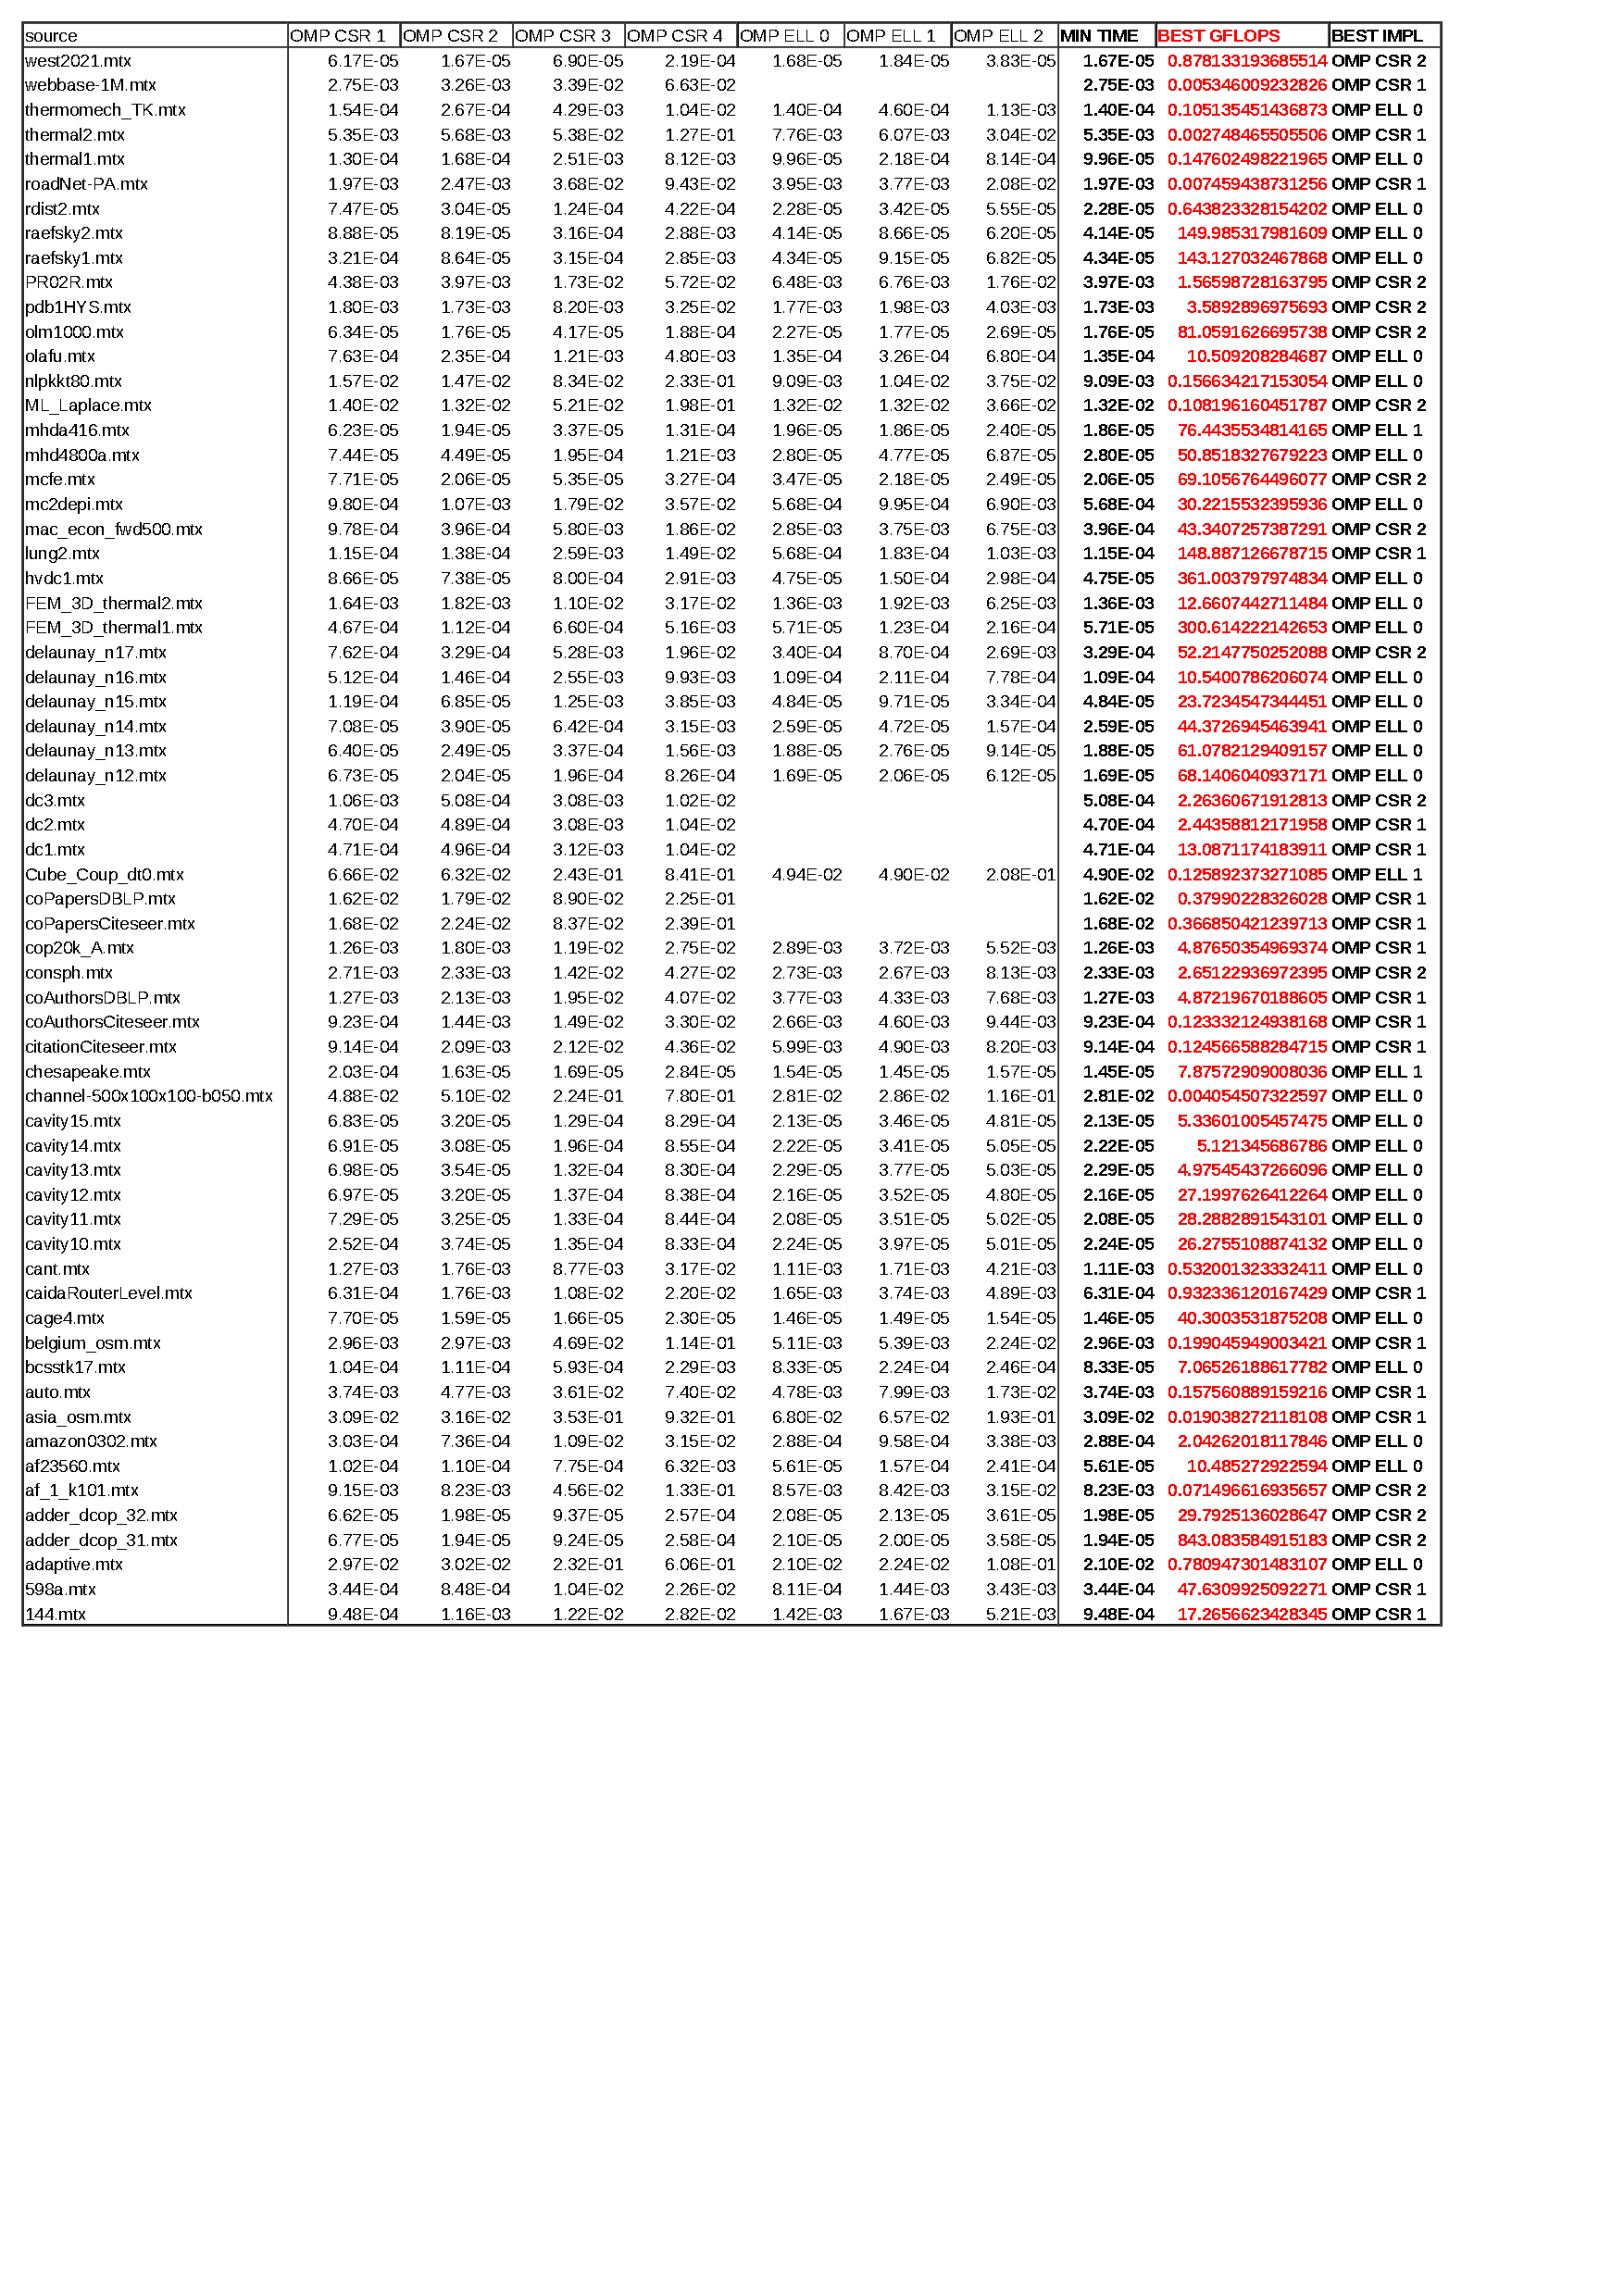
\includegraphics[width=\textwidth,height=\textheight,keepaspectratio=true]{ompNew_10x4_RL_NOSIMD_ImplConfrontoOut.pdf}
	%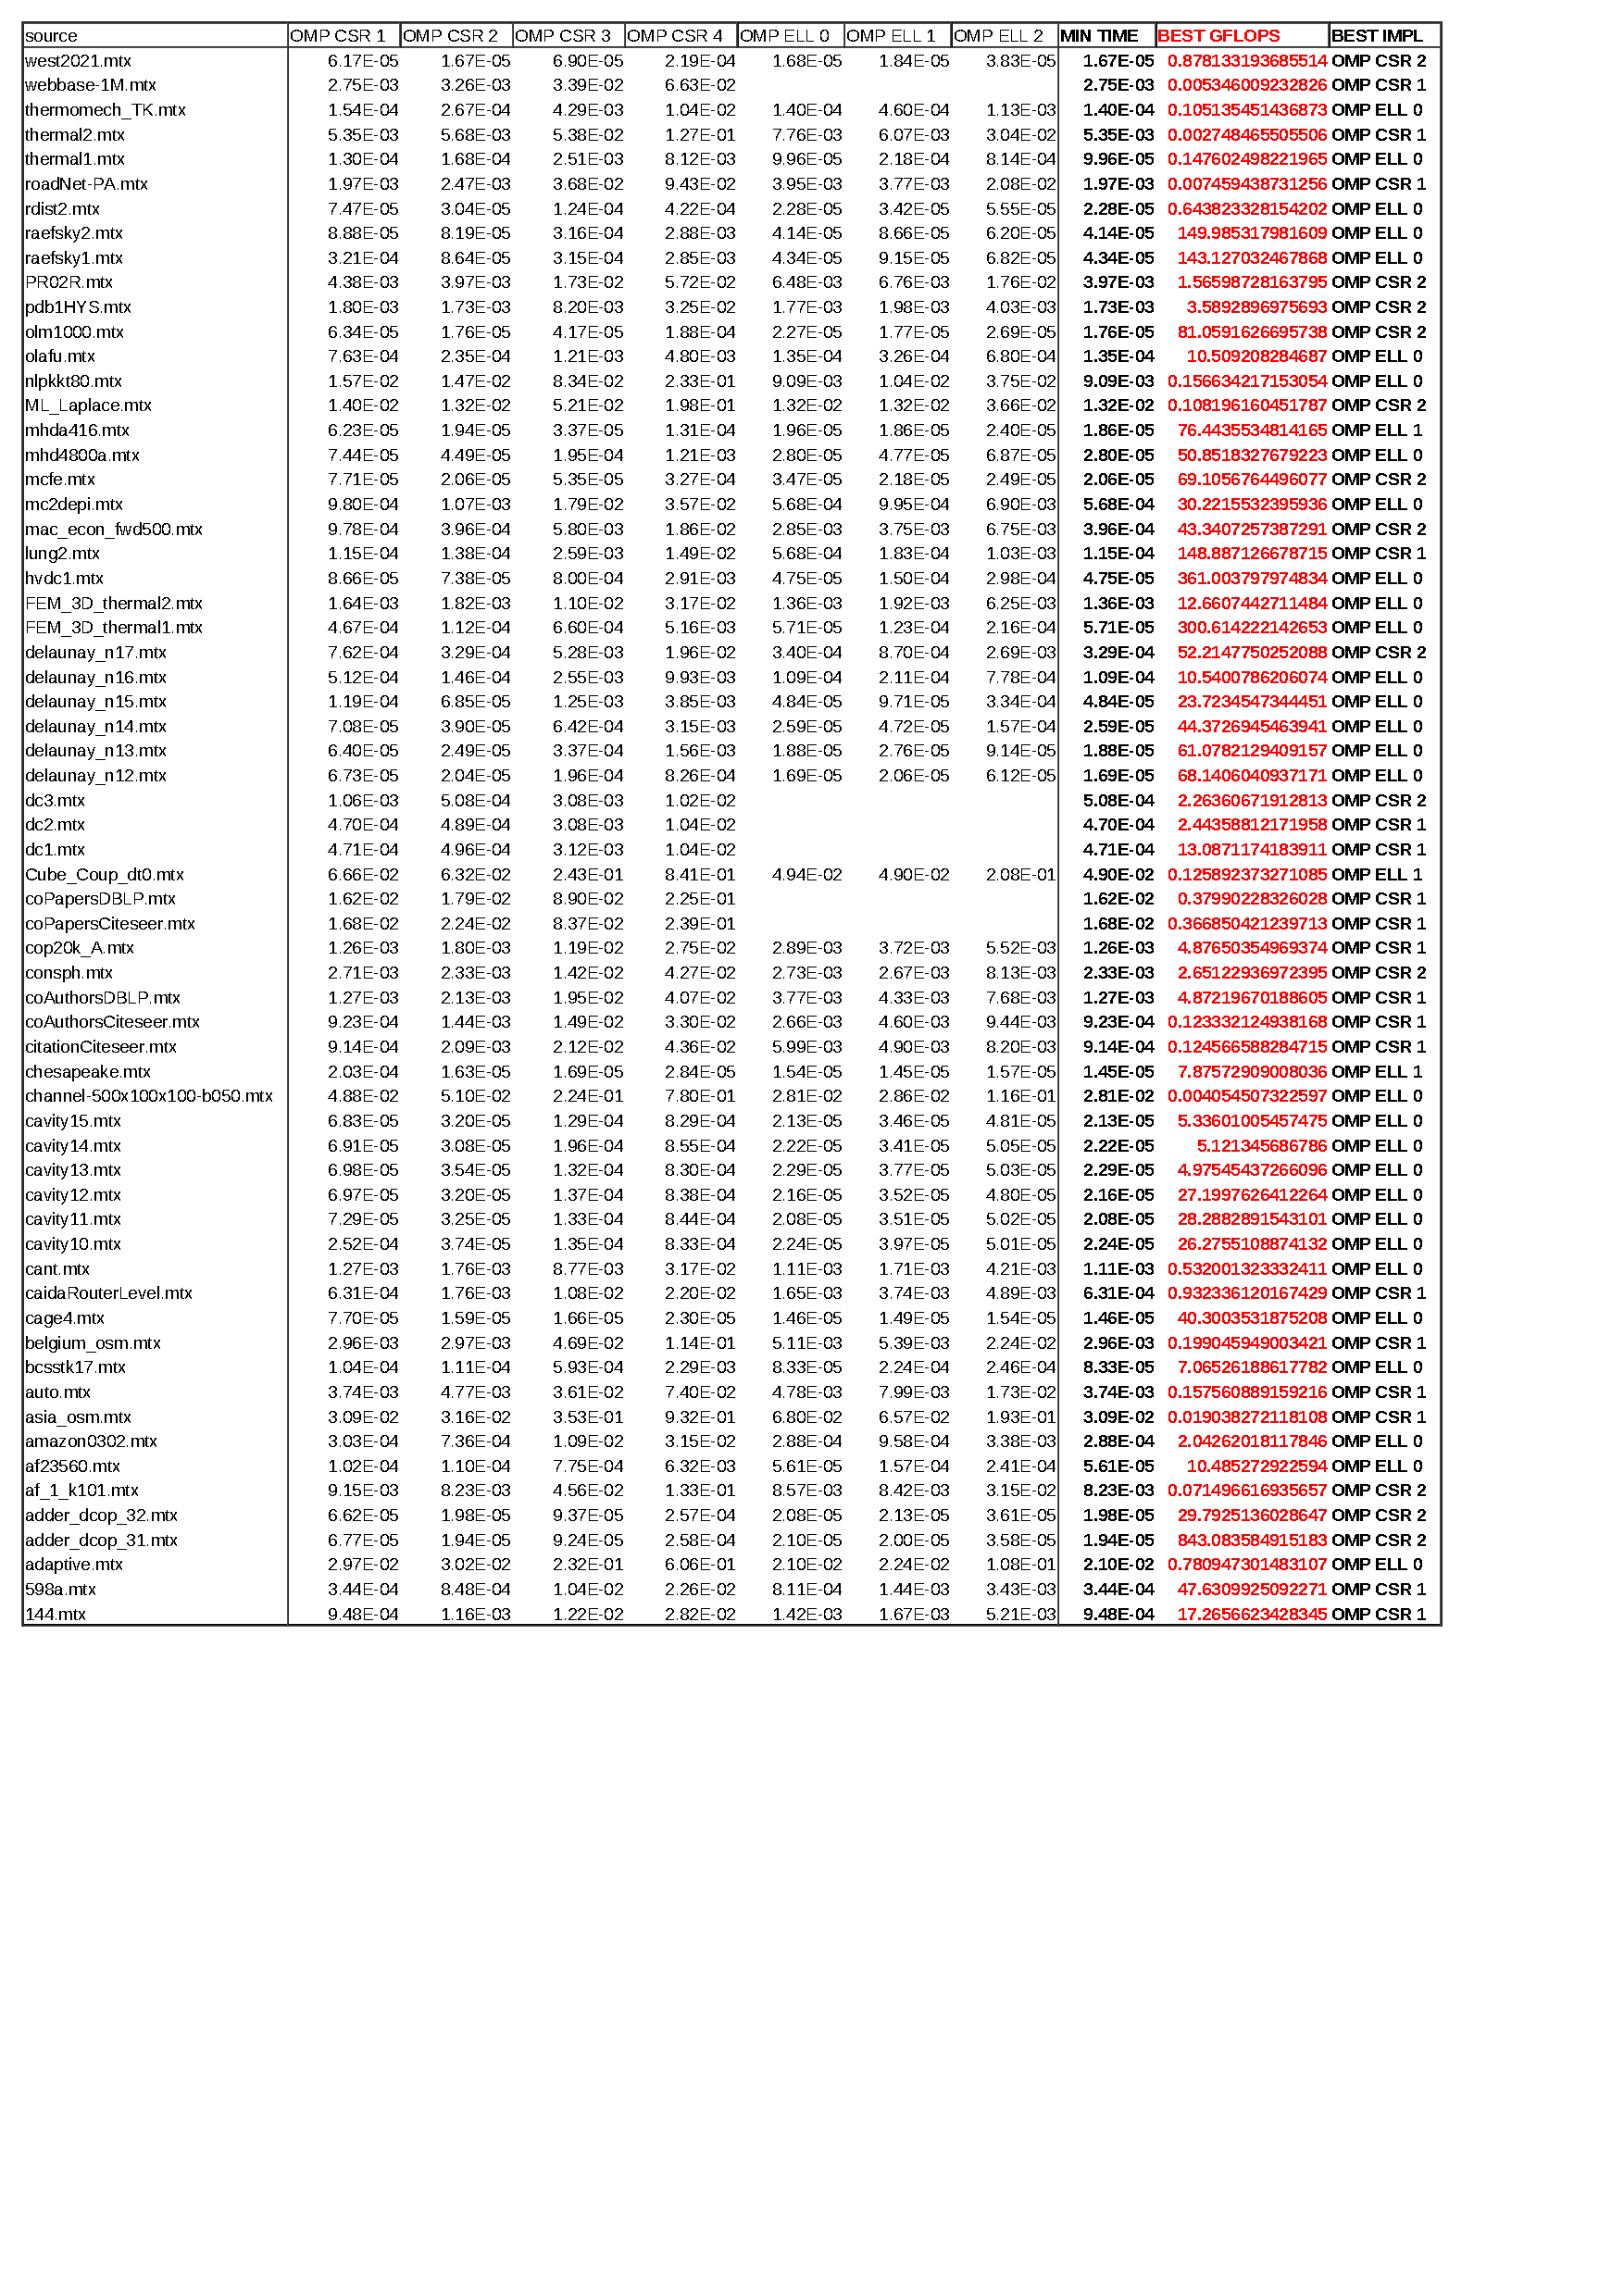
\includegraphics[scale=0.27]{ompNew_10x4_RL_NOSIMD_ImplConfrontoOut.pdf}
	\begin{figure}[h!]  \centering
        %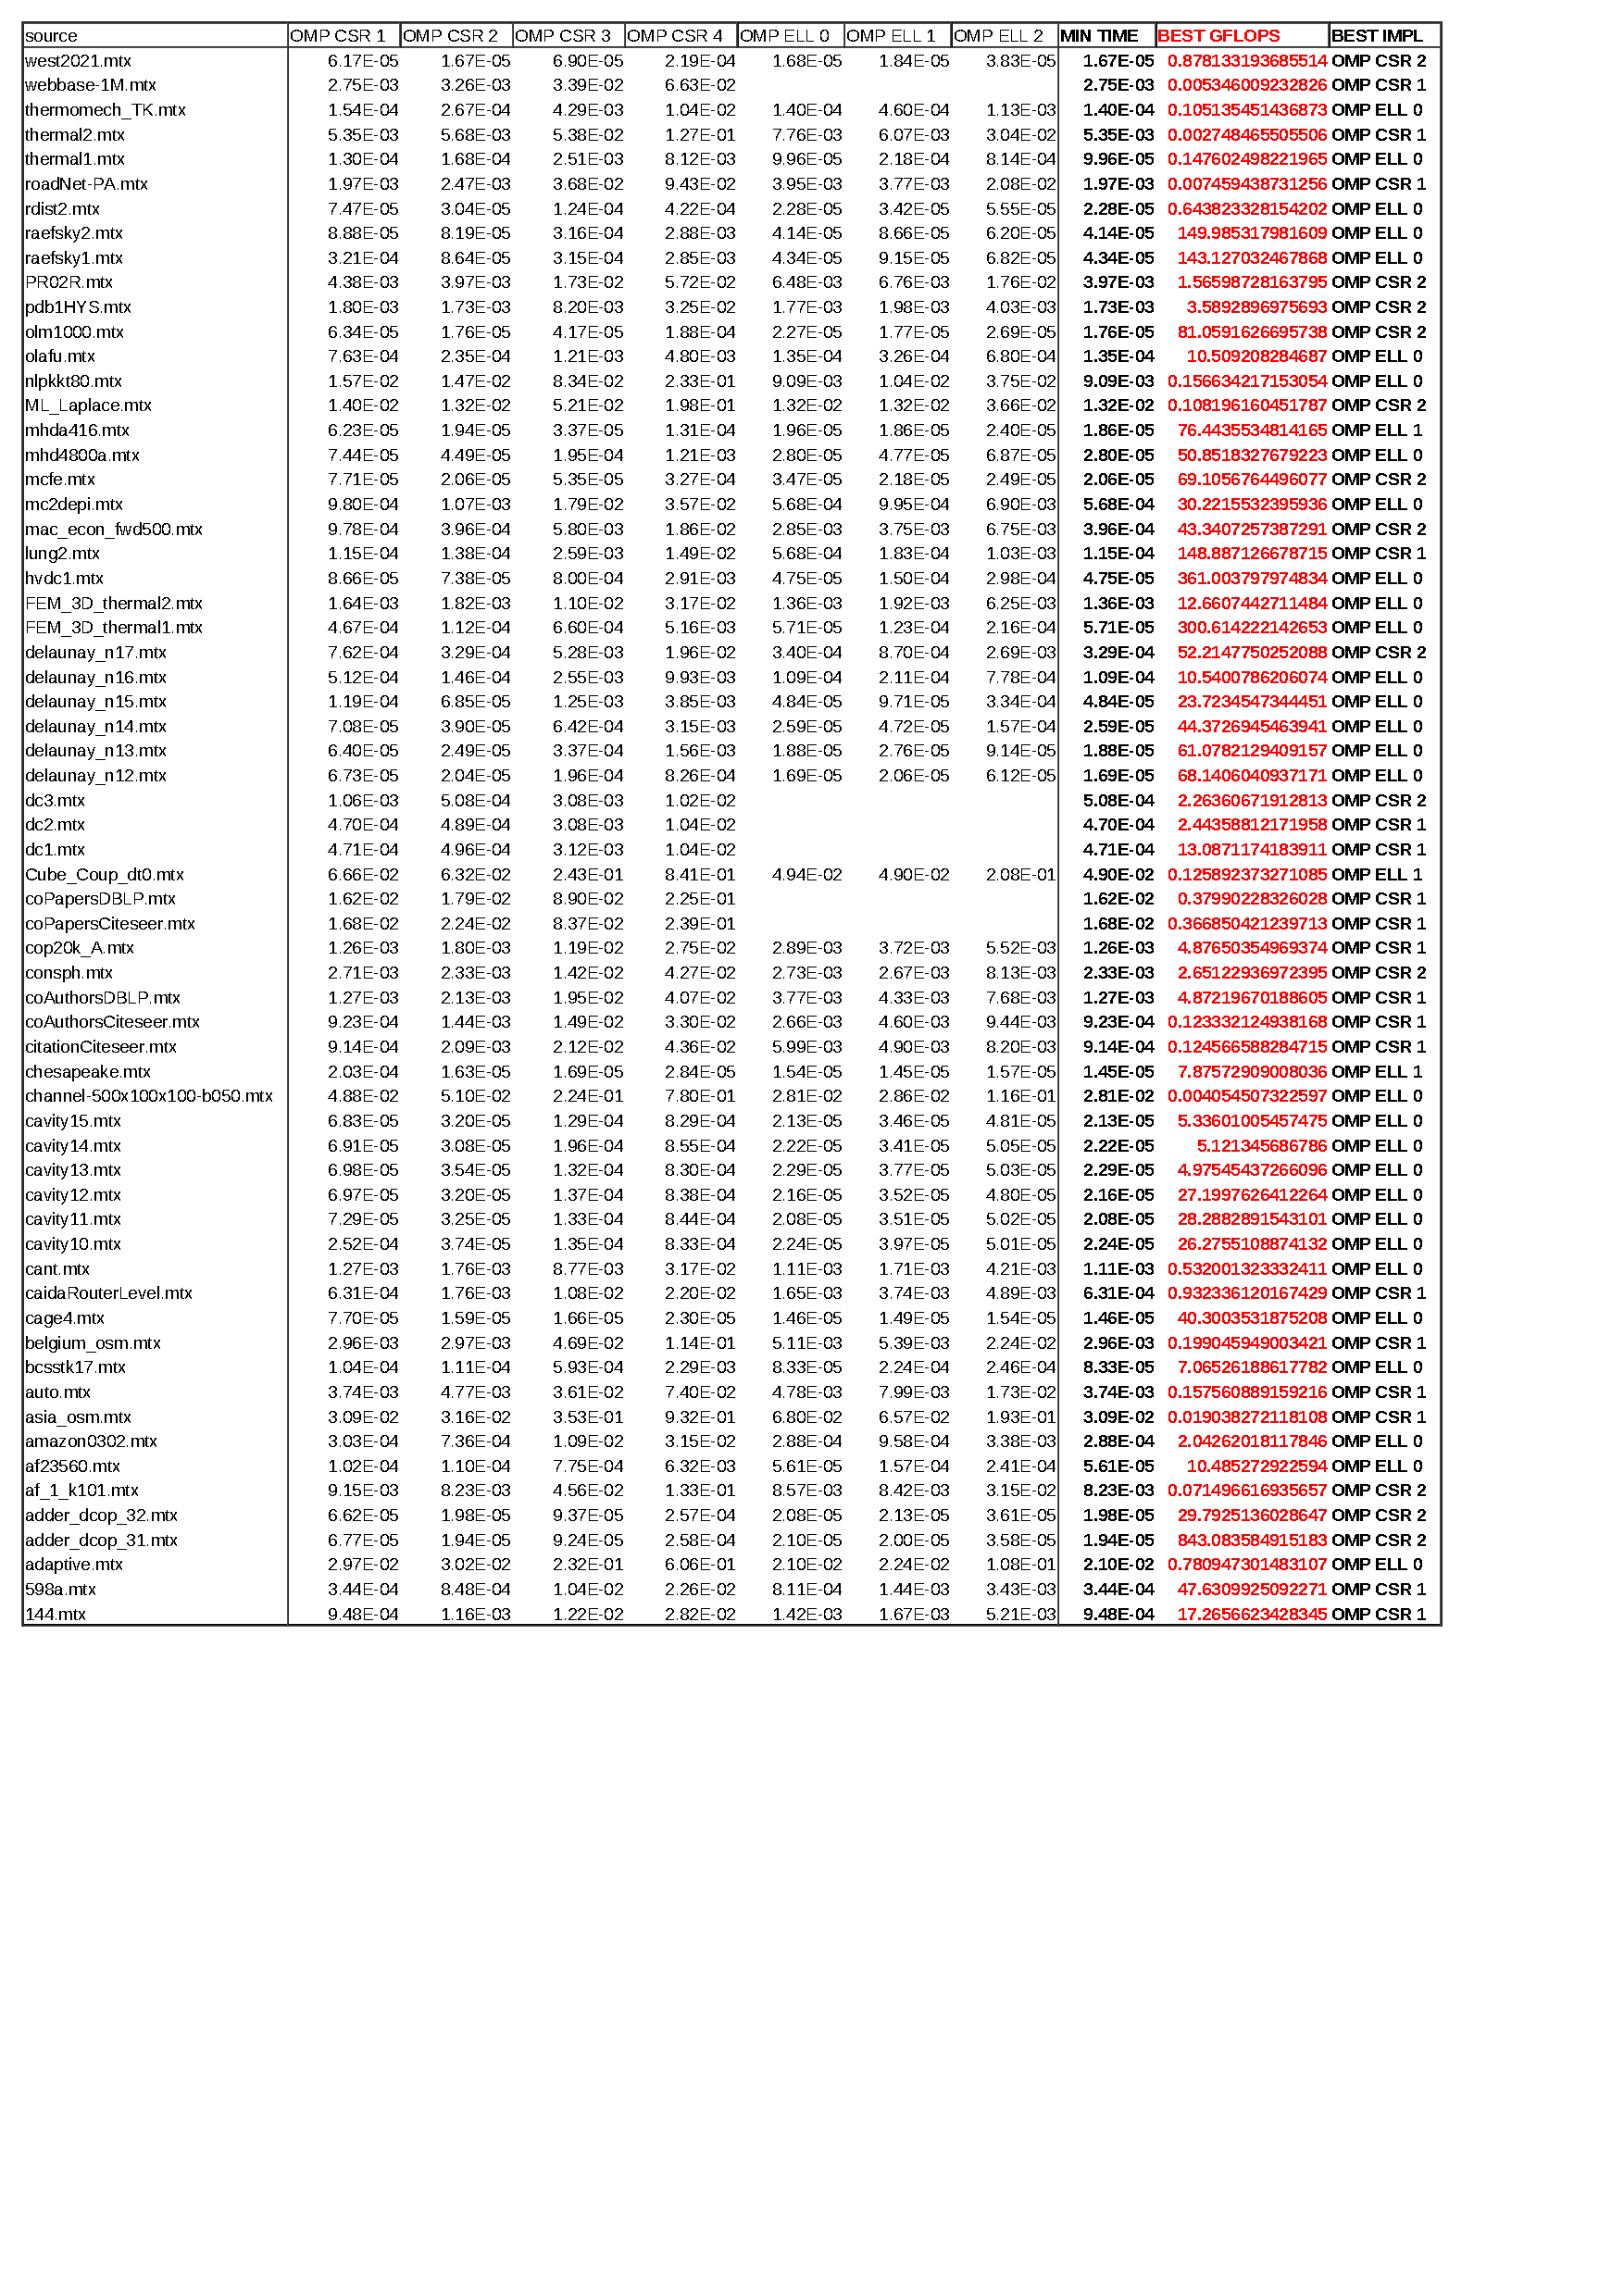
\includegraphics[width=\textwidth,height=\textheight,keepaspectratio=true]{ompNew_10x4_RL_NOSIMD_ImplConfrontoOut.pdf}
        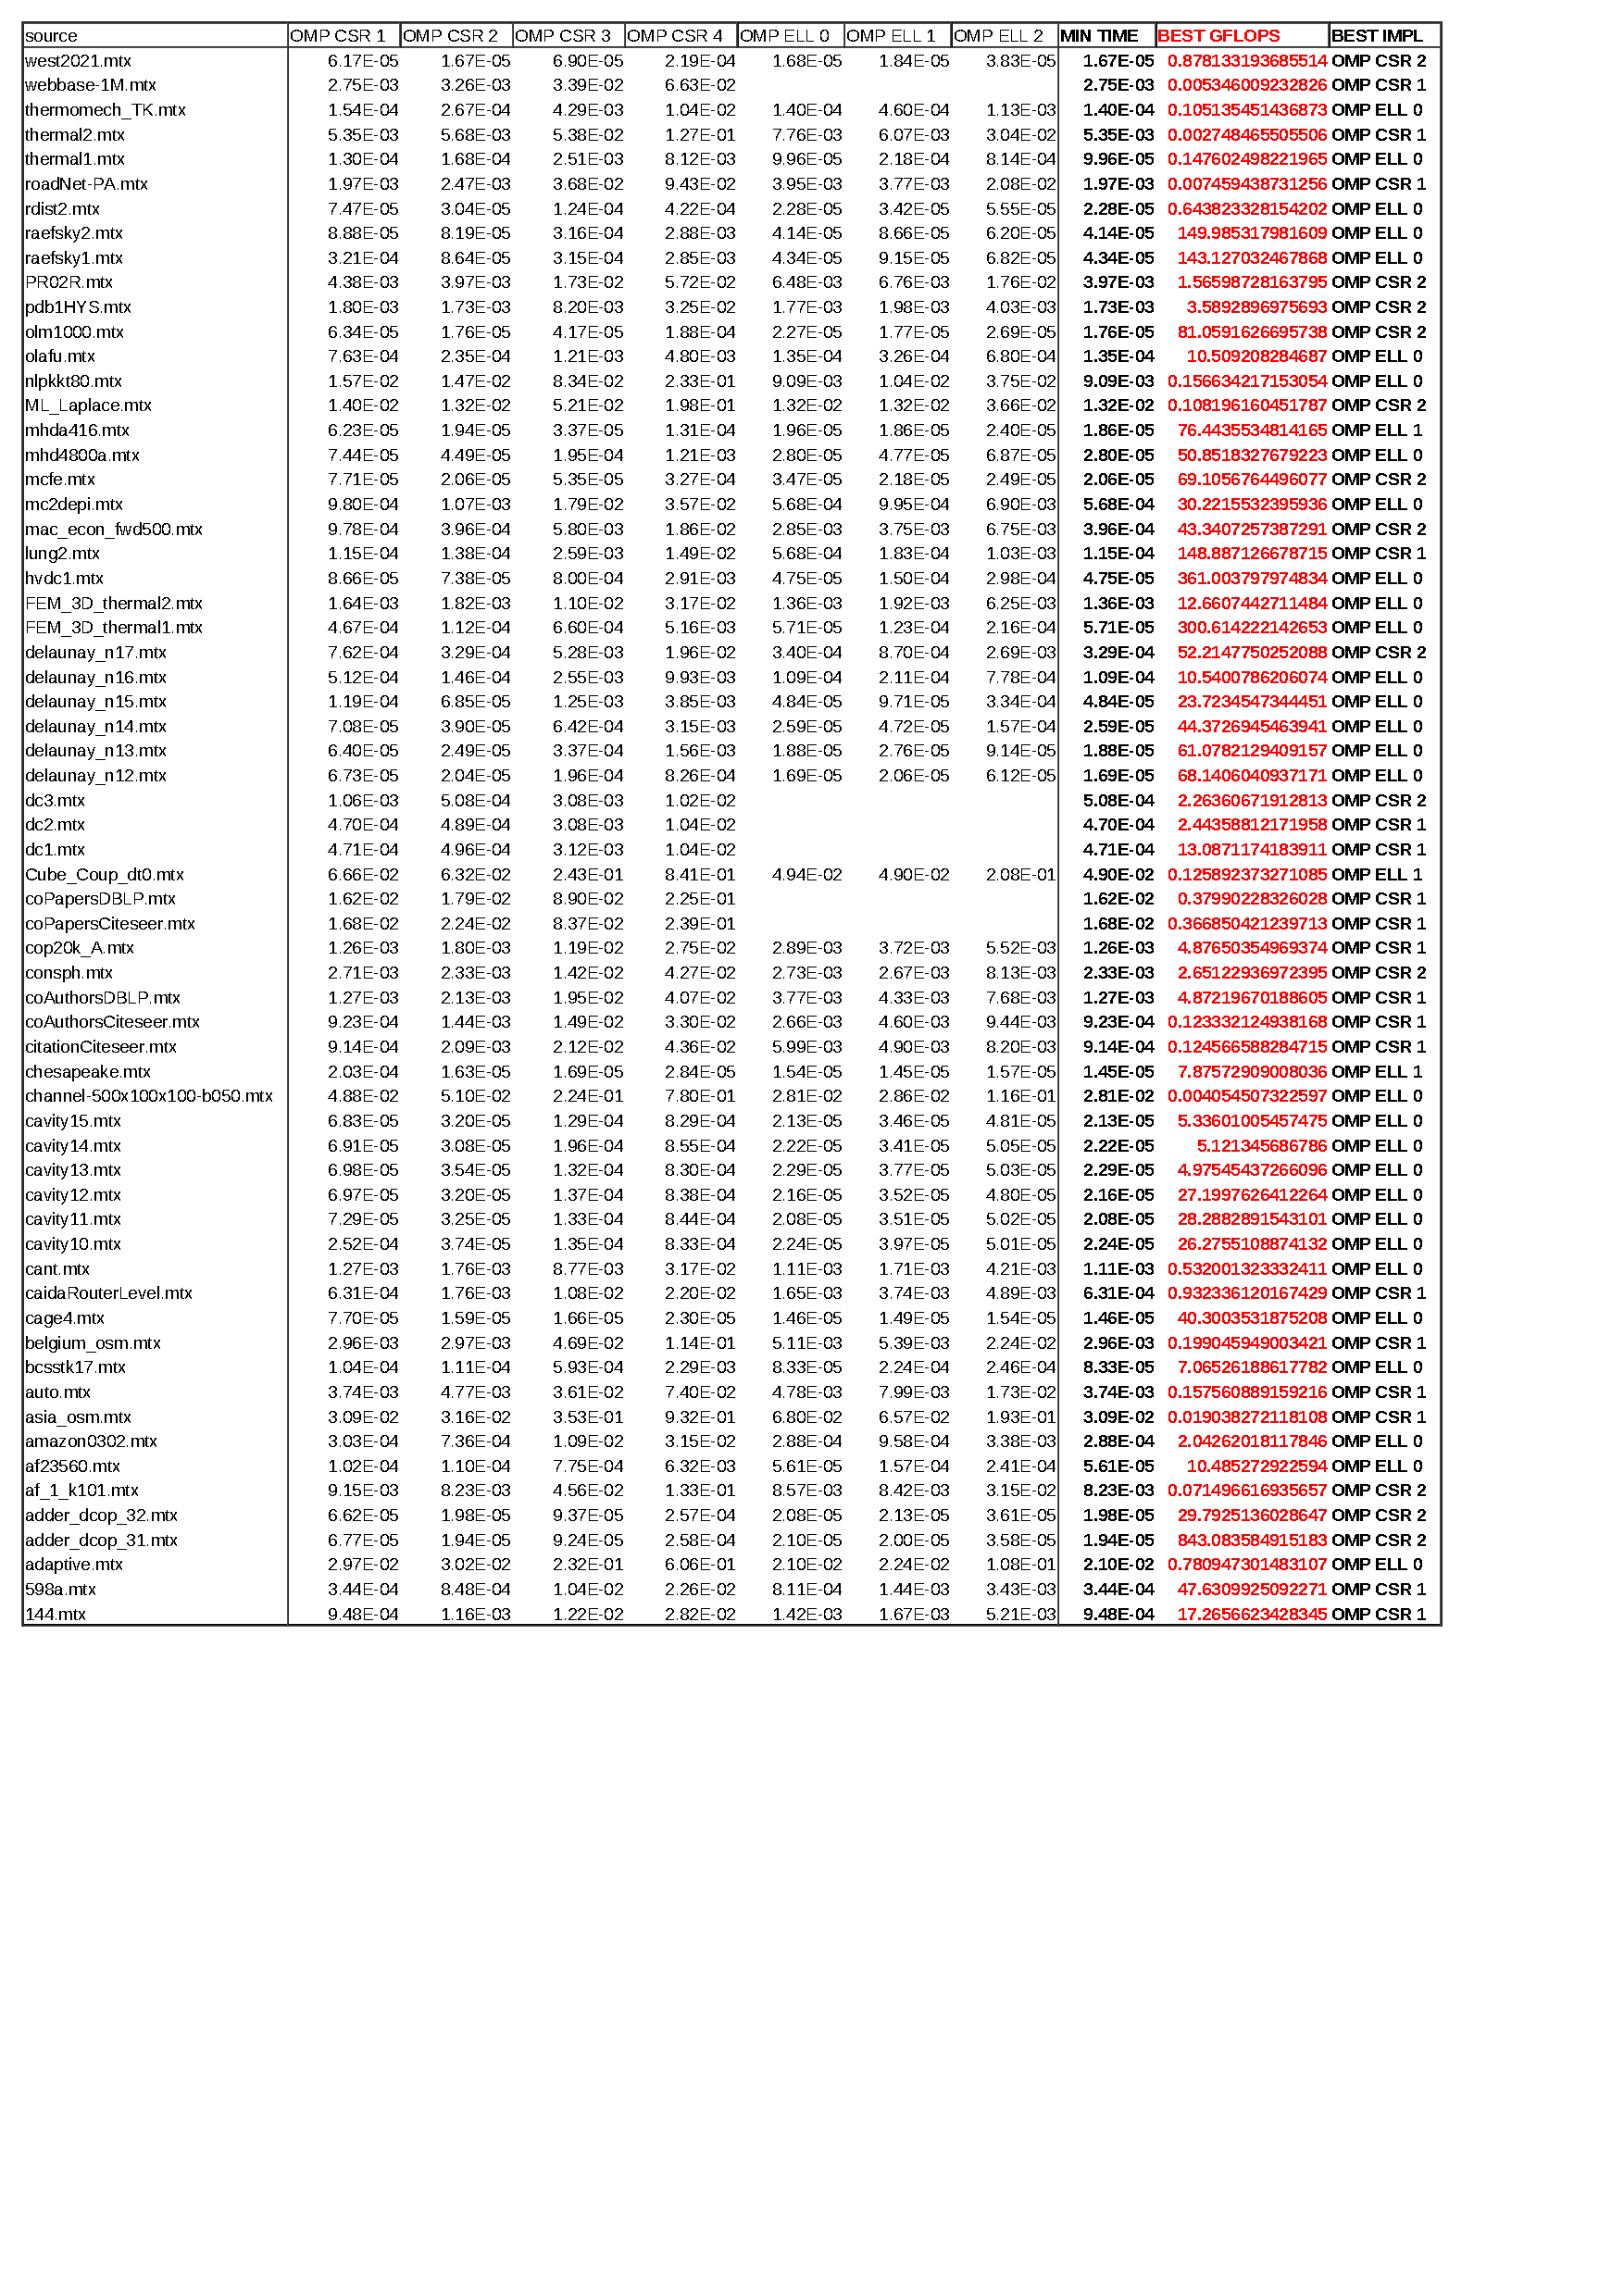
\includegraphics[scale=0.27]{ompNew_10x4_RL_NOSIMD_ImplConfrontoOut.pdf}
        %\caption{pdf centering + width+height}
    \end{figure}
\end{frame}

\subsection{CUDA}
\begin{frame}{Analisi performance CUDA}
	\begin{enumerate}
		\item	vettore ausiliario ROWLENS: svantaggio nel 55.96\% dei casi\\
				senza dare significativi cambiamenti ai tempi di esecuzione.\\
				Probabilmente per via della divergenza intra-warp introdotta 
		\pause
		\item	Dimensionamento dei blocchi per il lancio dei kernel\\
				configurazioni analizzate:
		\pause
		\begin{enumerate}
			\item	blocchi 1D per le implementazioni con 1 thread per riga di:\\192, 256 e 384
			\item	blocchi 2D per le implementazioni con 1 warp per riga di 32x\\8,16,32
		\end{enumerate}
		\item	Configurazioni con performance migliori su 
				tutte le implementazioni per ogni matrice\\
				(senza il vettore ausiliario ROWLENS)
		\pause
		\begin{itemize}
			\item 192 e 32x8  nel 58.09\% dei casi
			\item 384 e 32x16 nel 34.32\% dei casi
			\item 256 e 32x32 nel  6.60\% dei casi
		\end{itemize}
	\end{enumerate}
\end{frame}

\begin{frame}[t]{misurazioni CUDA, no ROWLENS, blocchi 192 e 32x8}
	%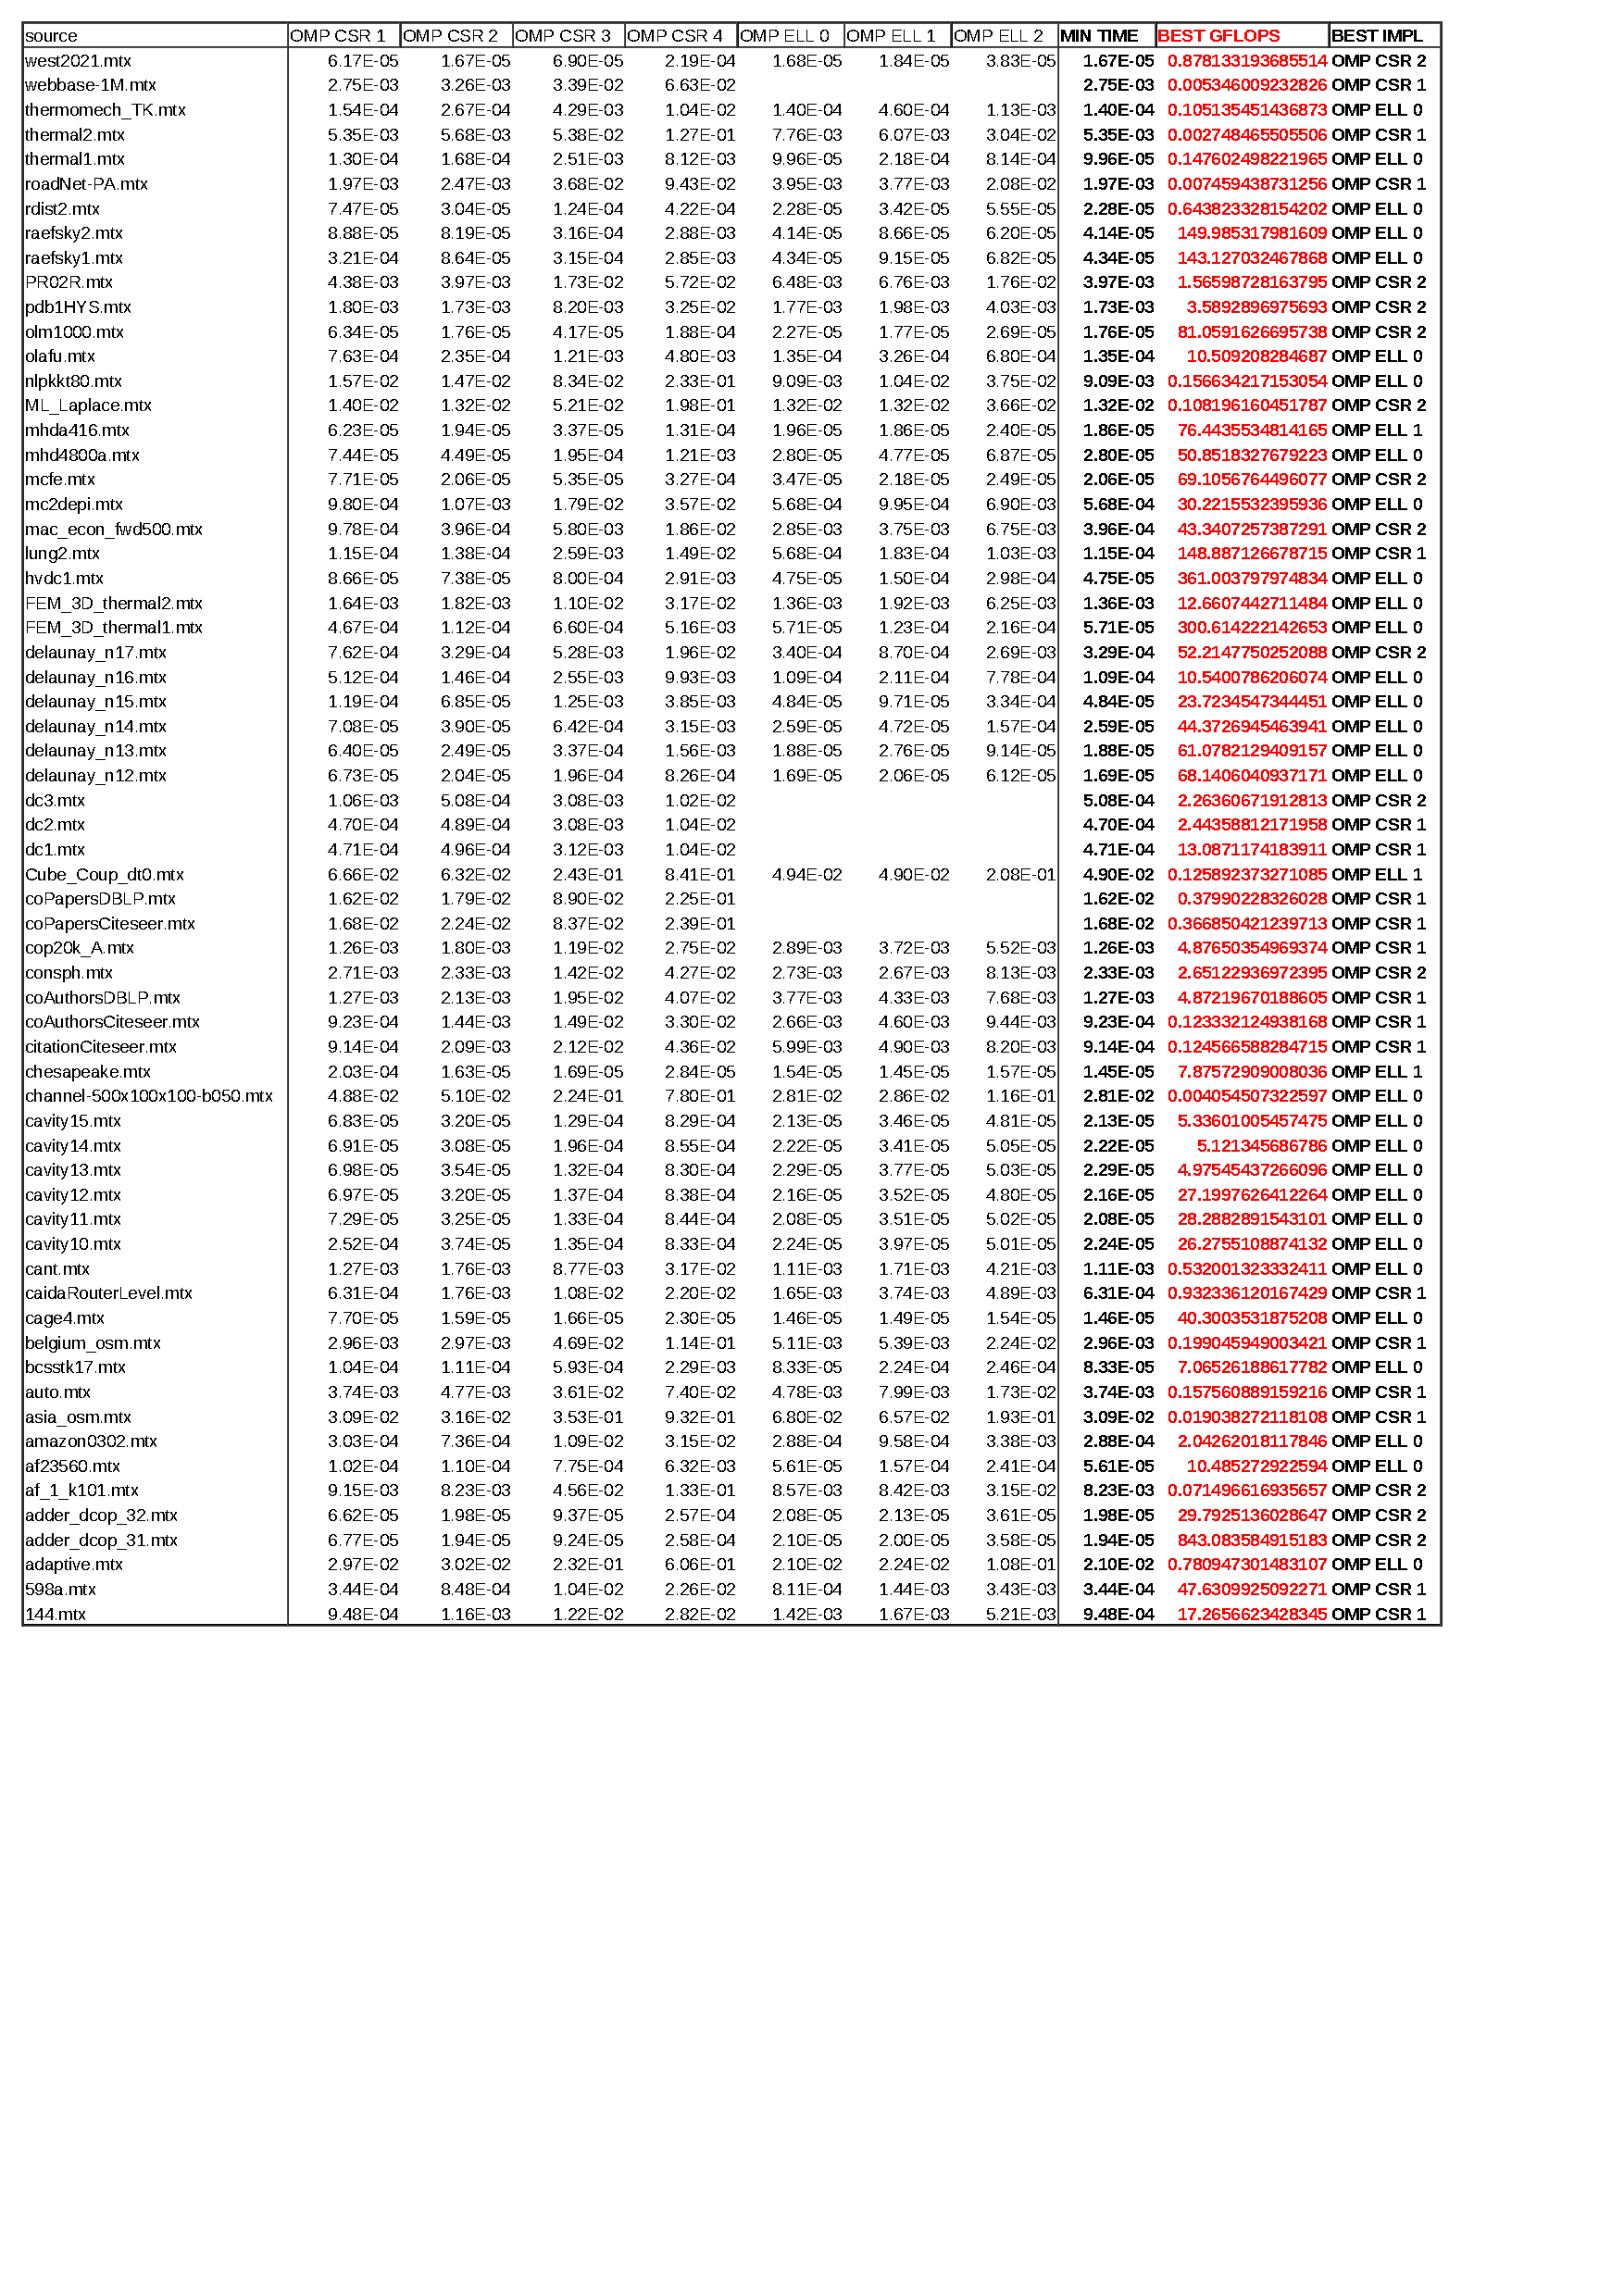
\includegraphics[width=\textwidth,height=\textheight,keepaspectratio=true]{ompNew_10x4_RL_NOSIMD_ImplConfrontoOut.pdf}
	%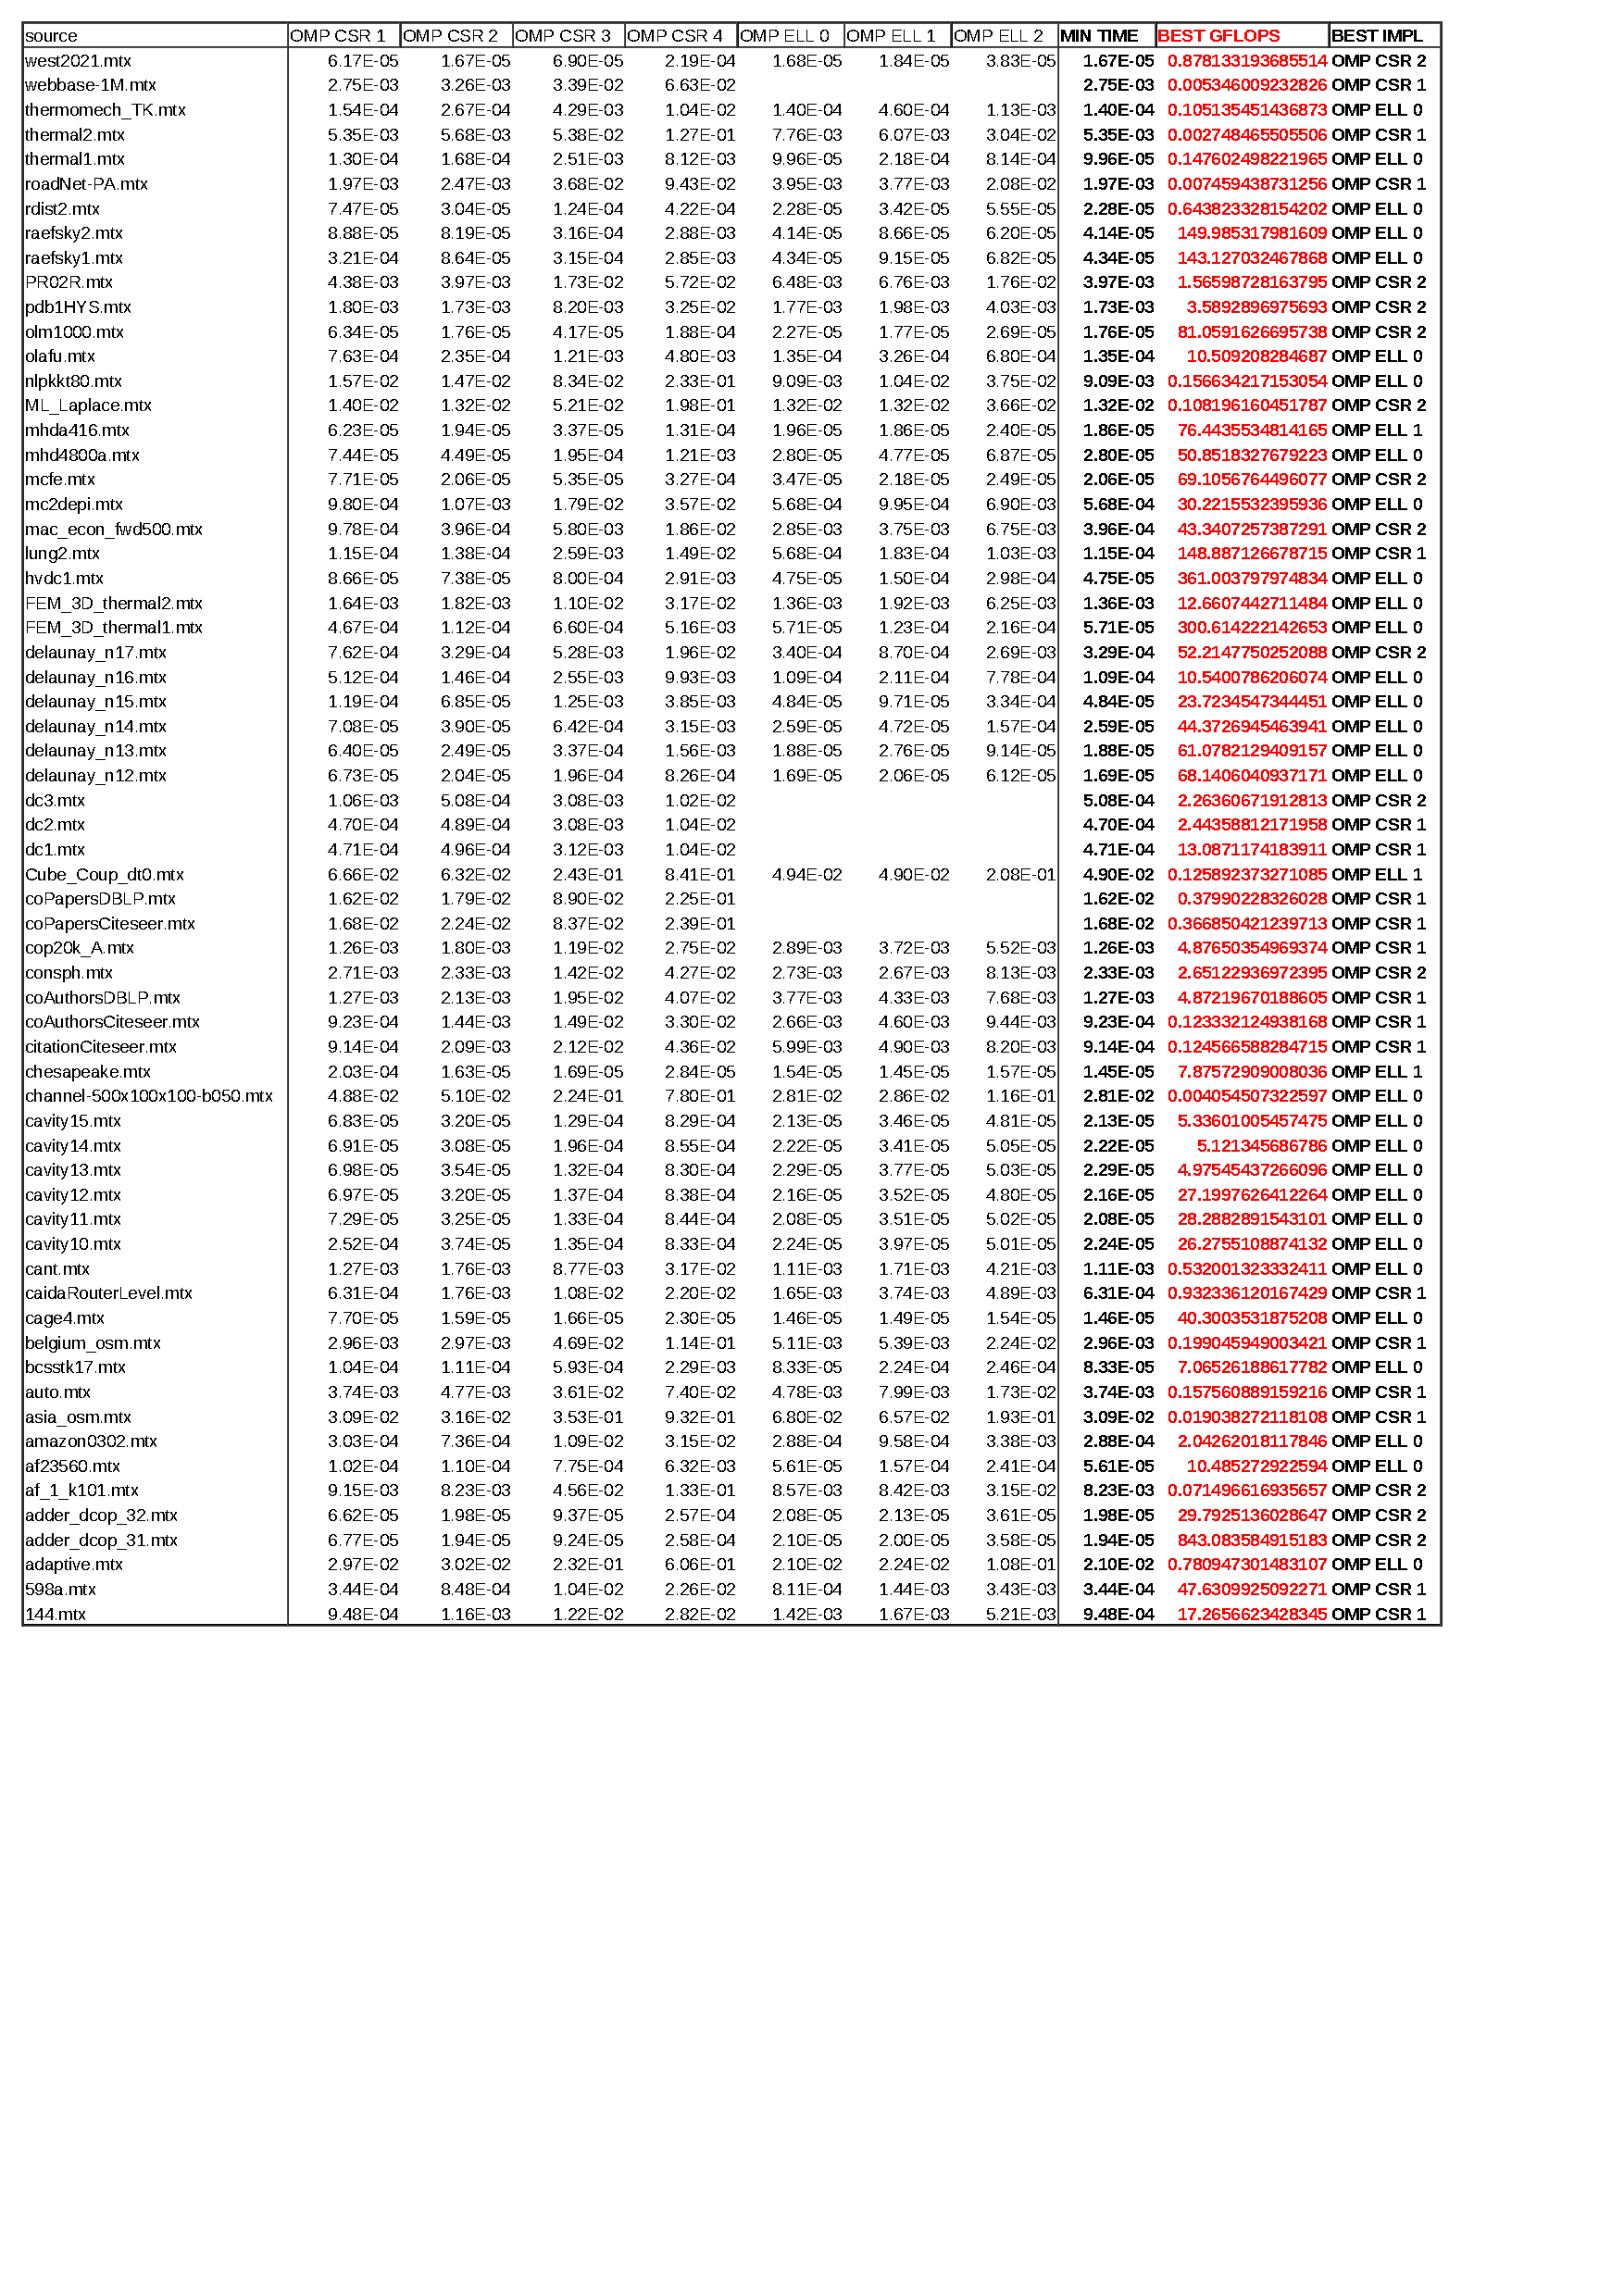
\includegraphics[scale=0.27]{ompNew_10x4_RL_NOSIMD_ImplConfrontoOut.pdf}
	\begin{figure}[h!]  \centering
        %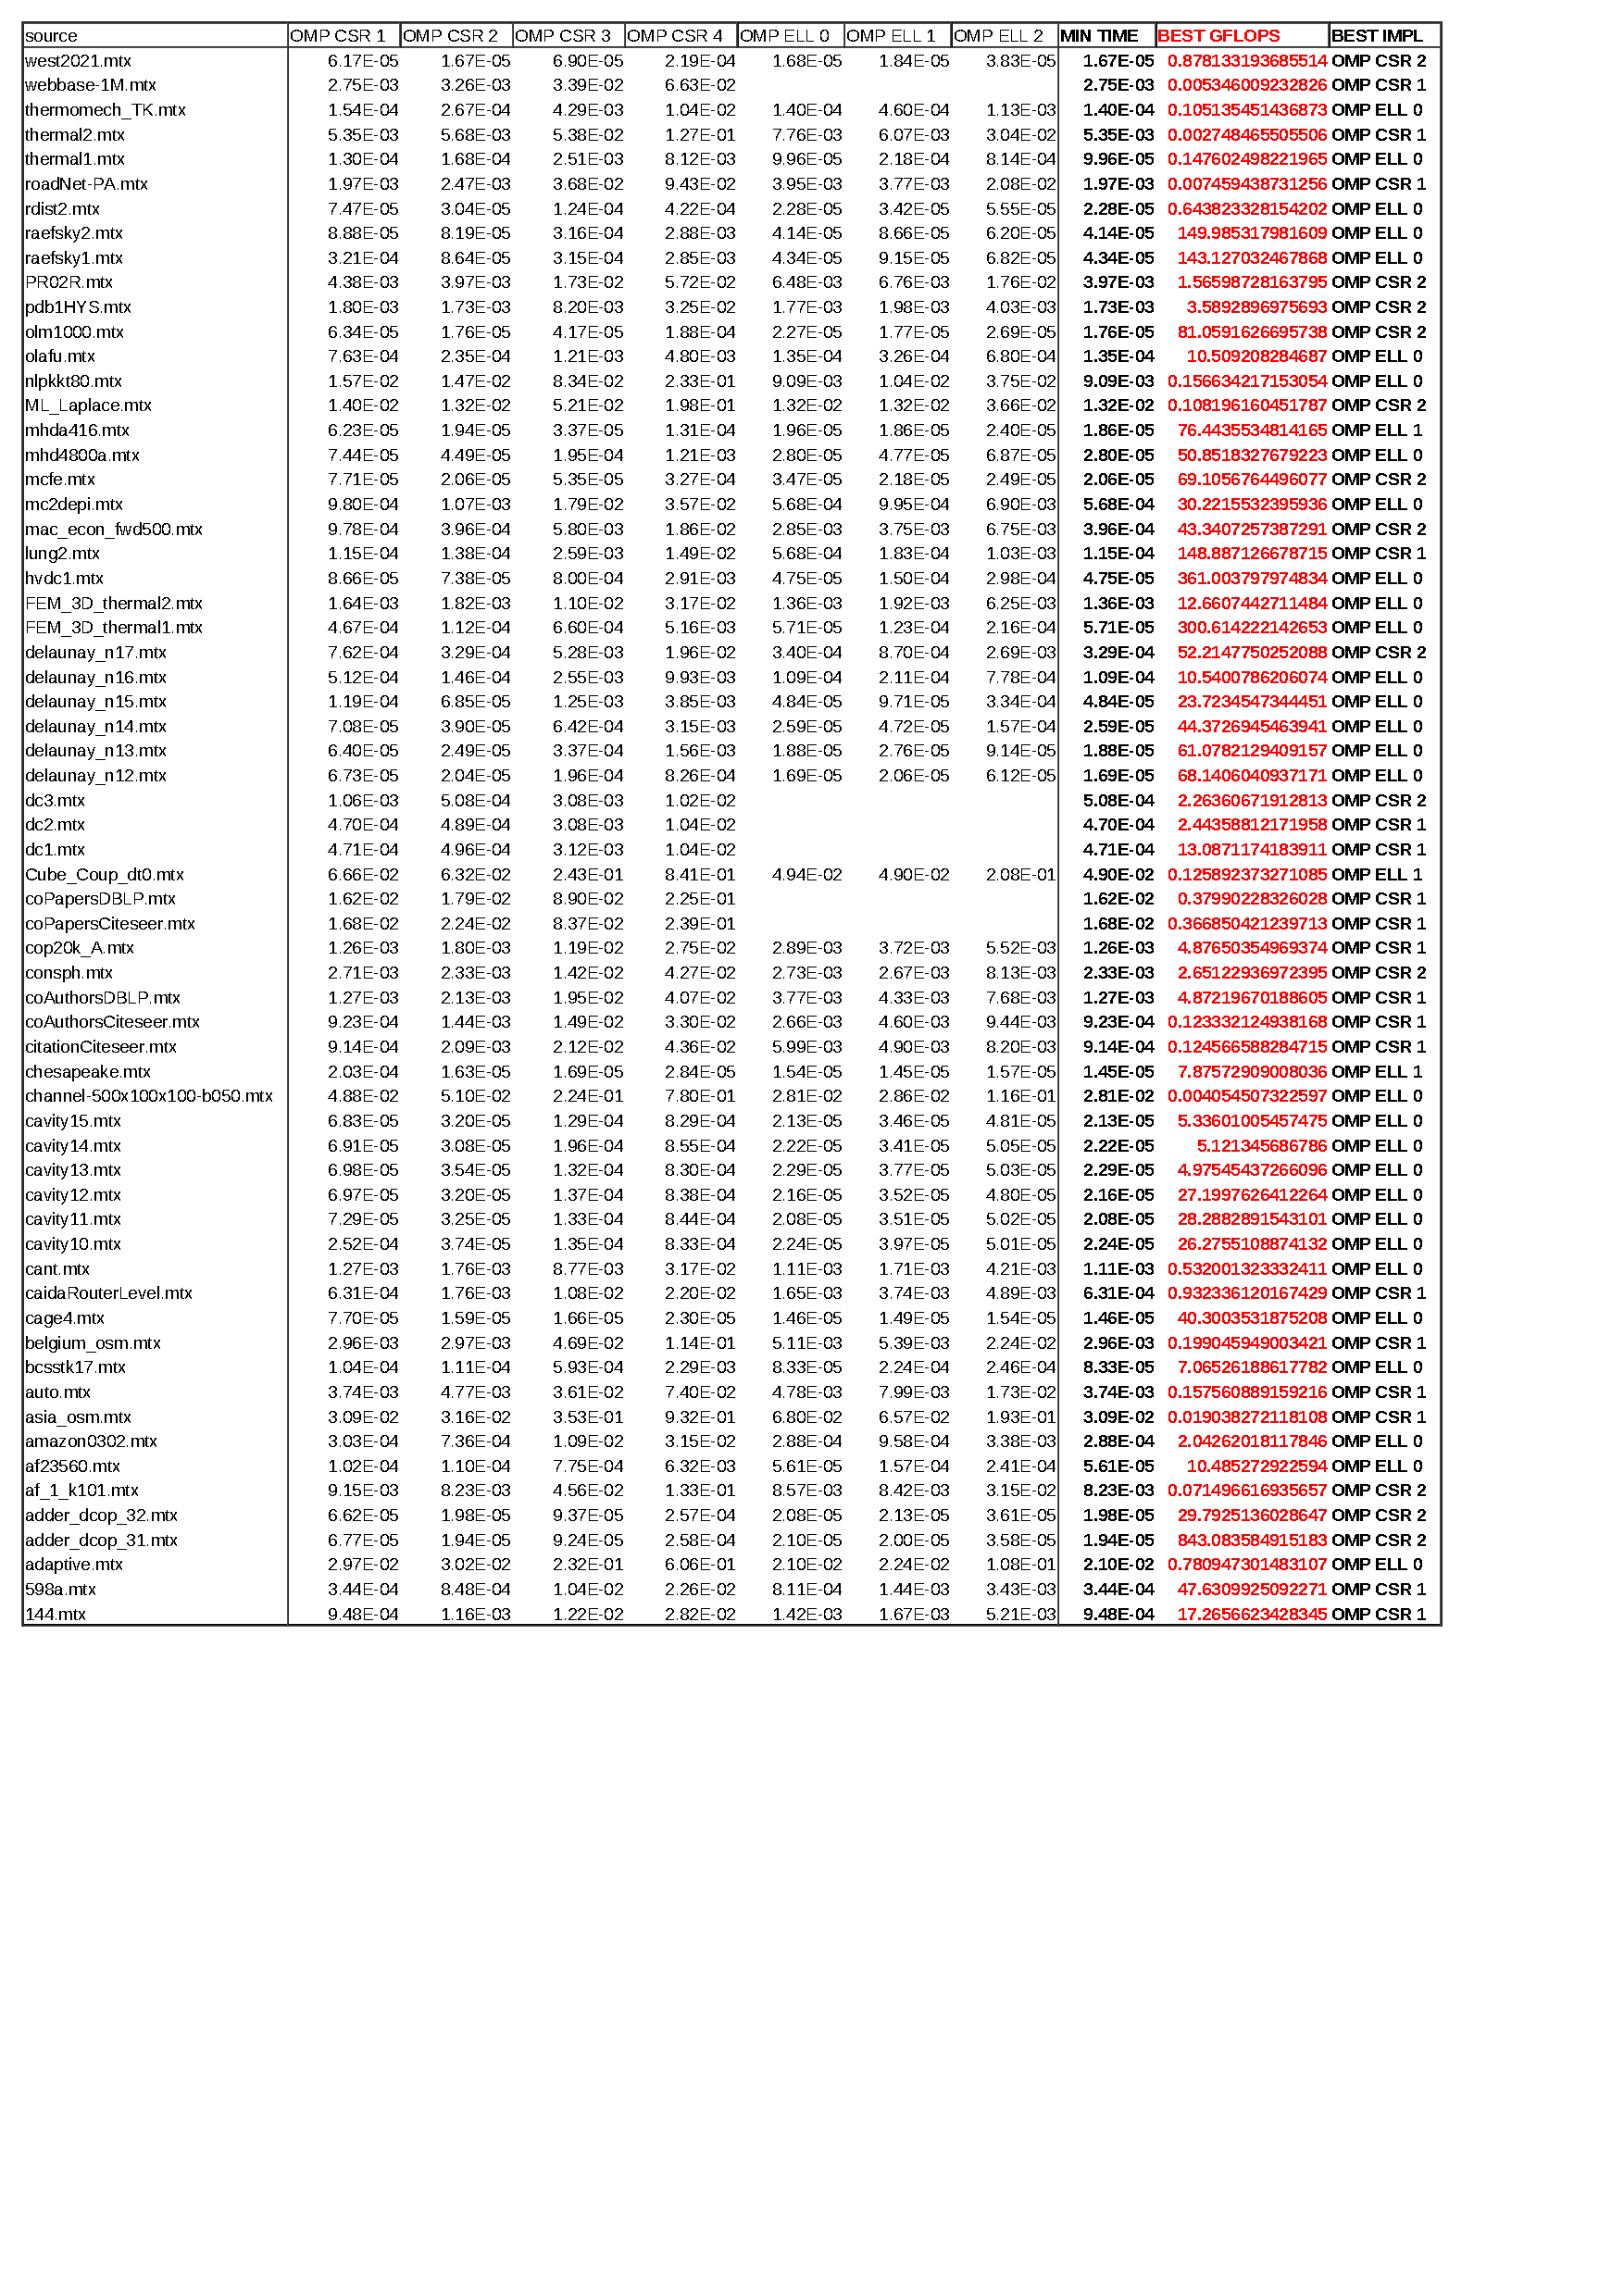
\includegraphics[width=\textwidth,height=\textheight,keepaspectratio=true]{ompNew_10x4_RL_NOSIMD_ImplConfrontoOut.pdf}
        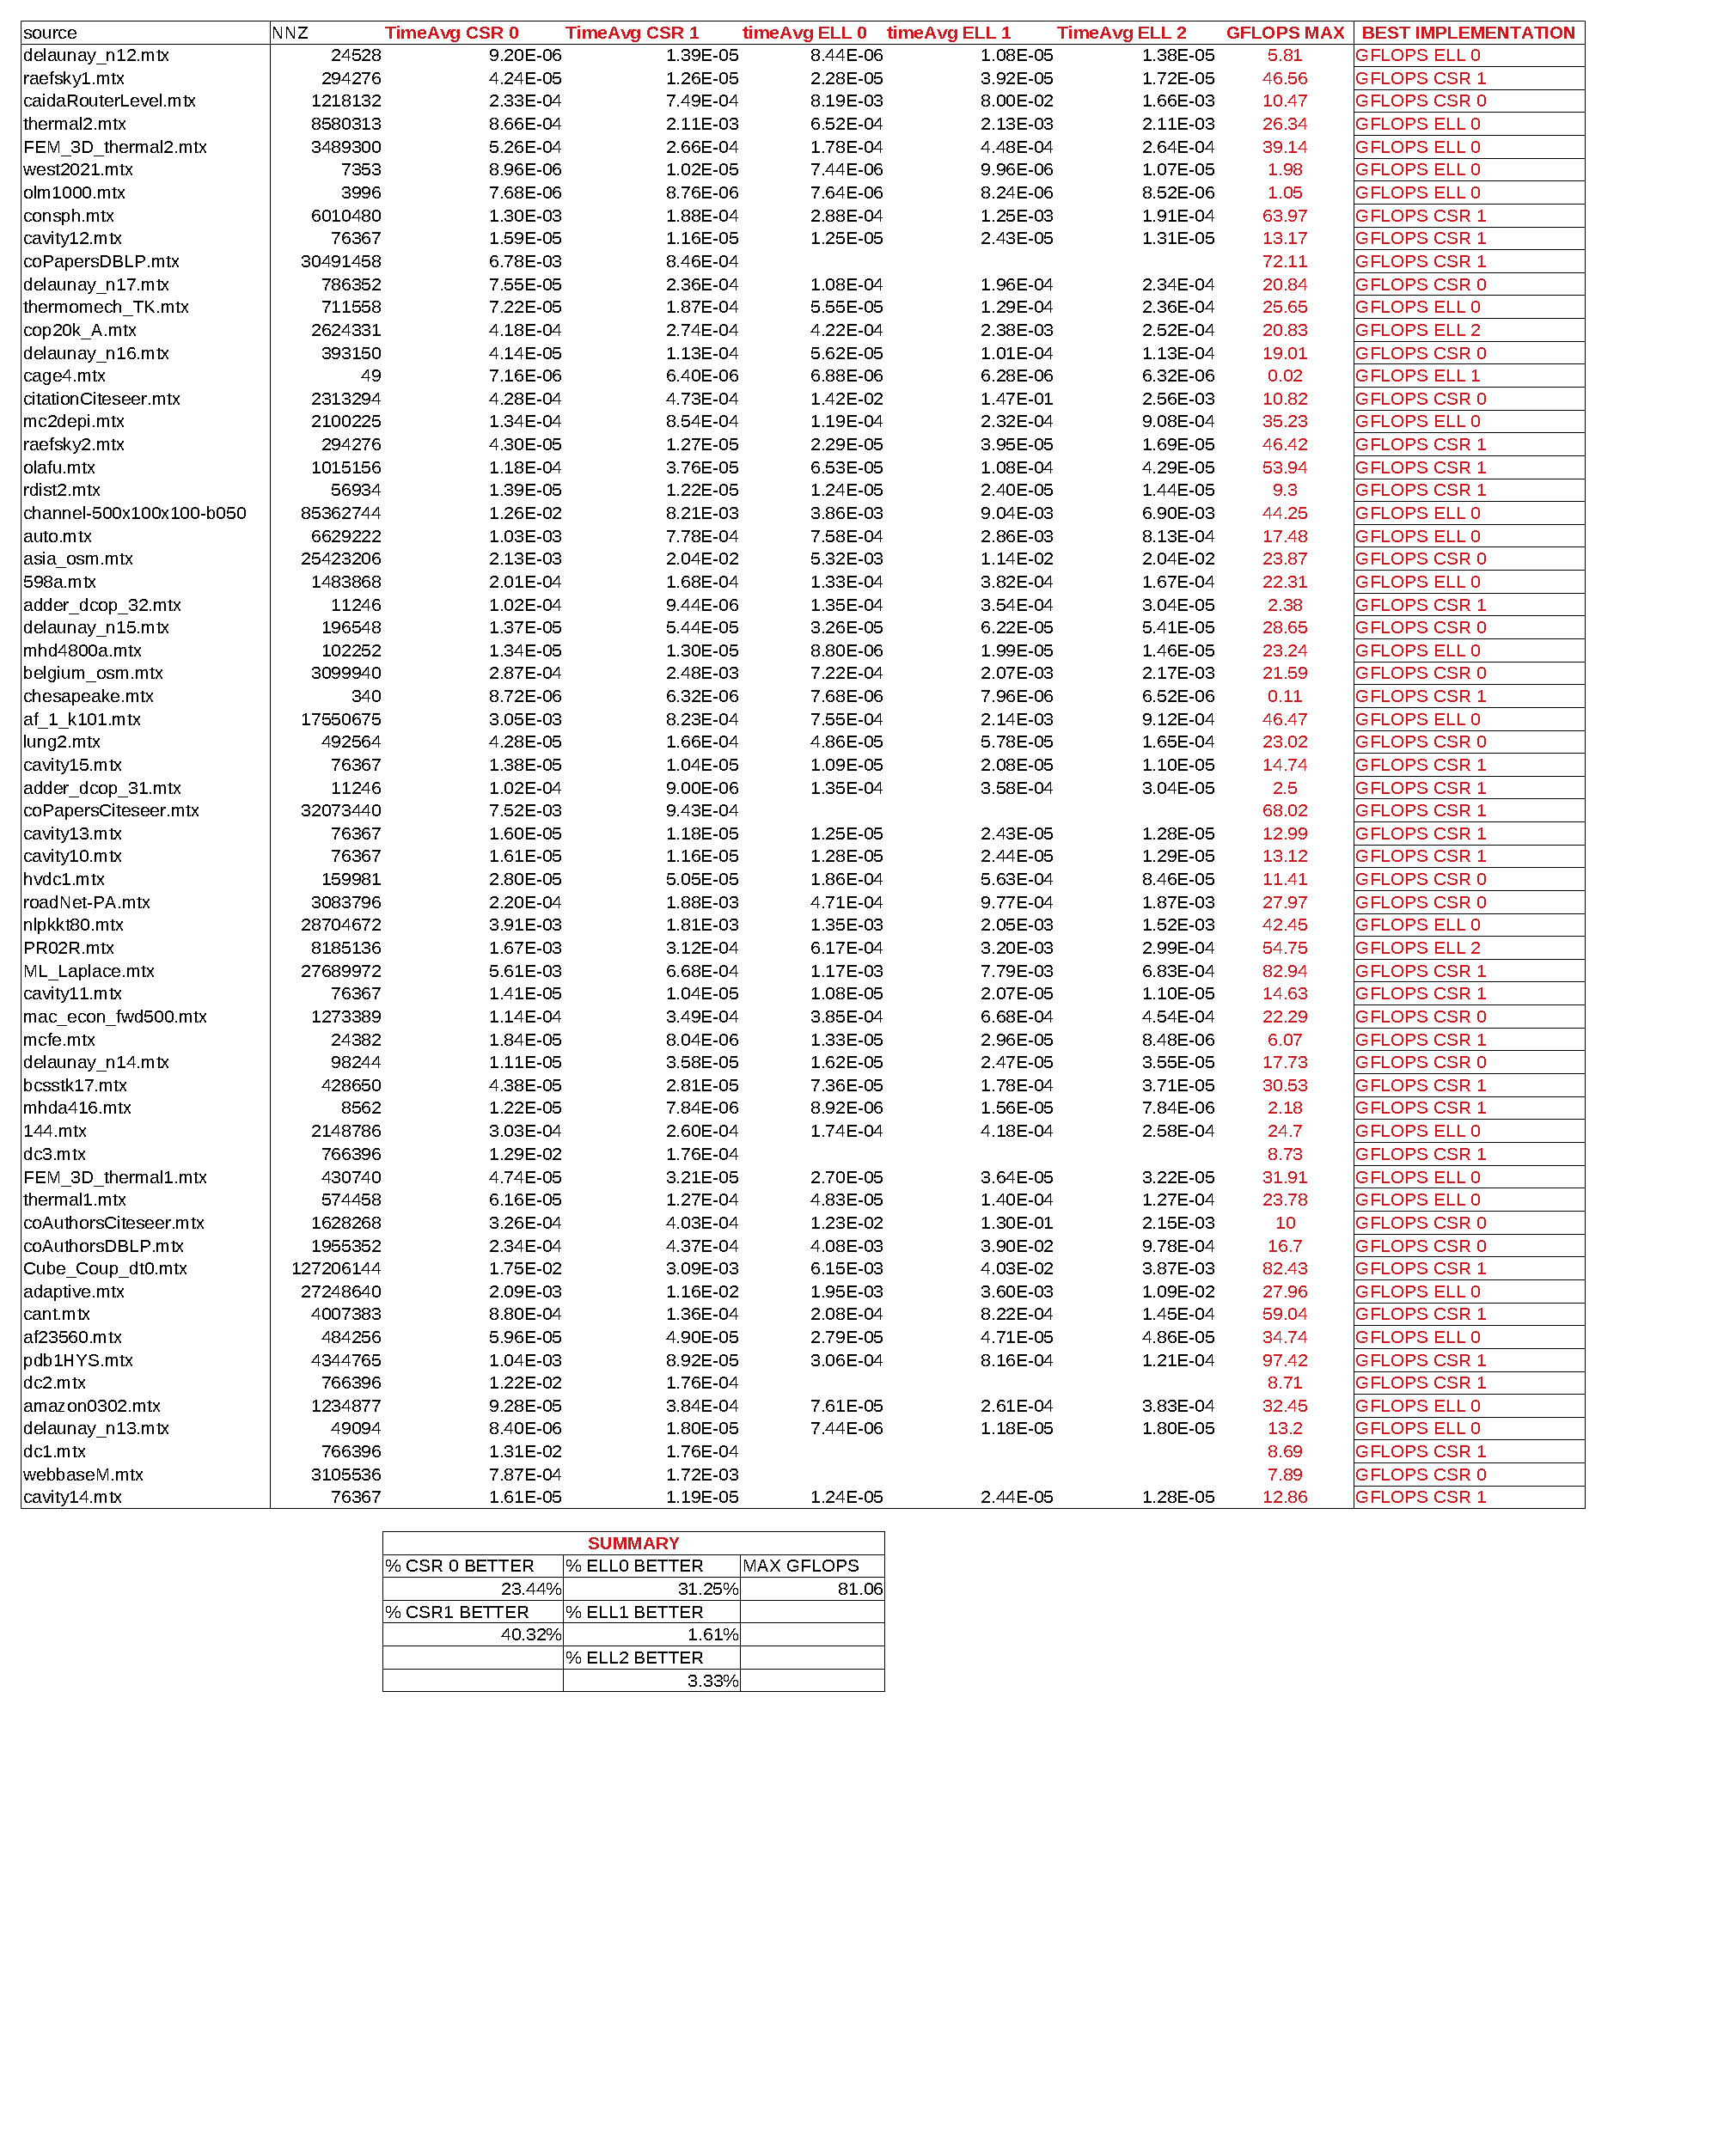
\includegraphics[scale=0.27]{cudaNoRowLens_192_8.pdf}
        %\caption{pdf centering + width+height}
    \end{figure}
\end{frame}

\begin{frame}[t]{Confronto CUDA - OMP}
	%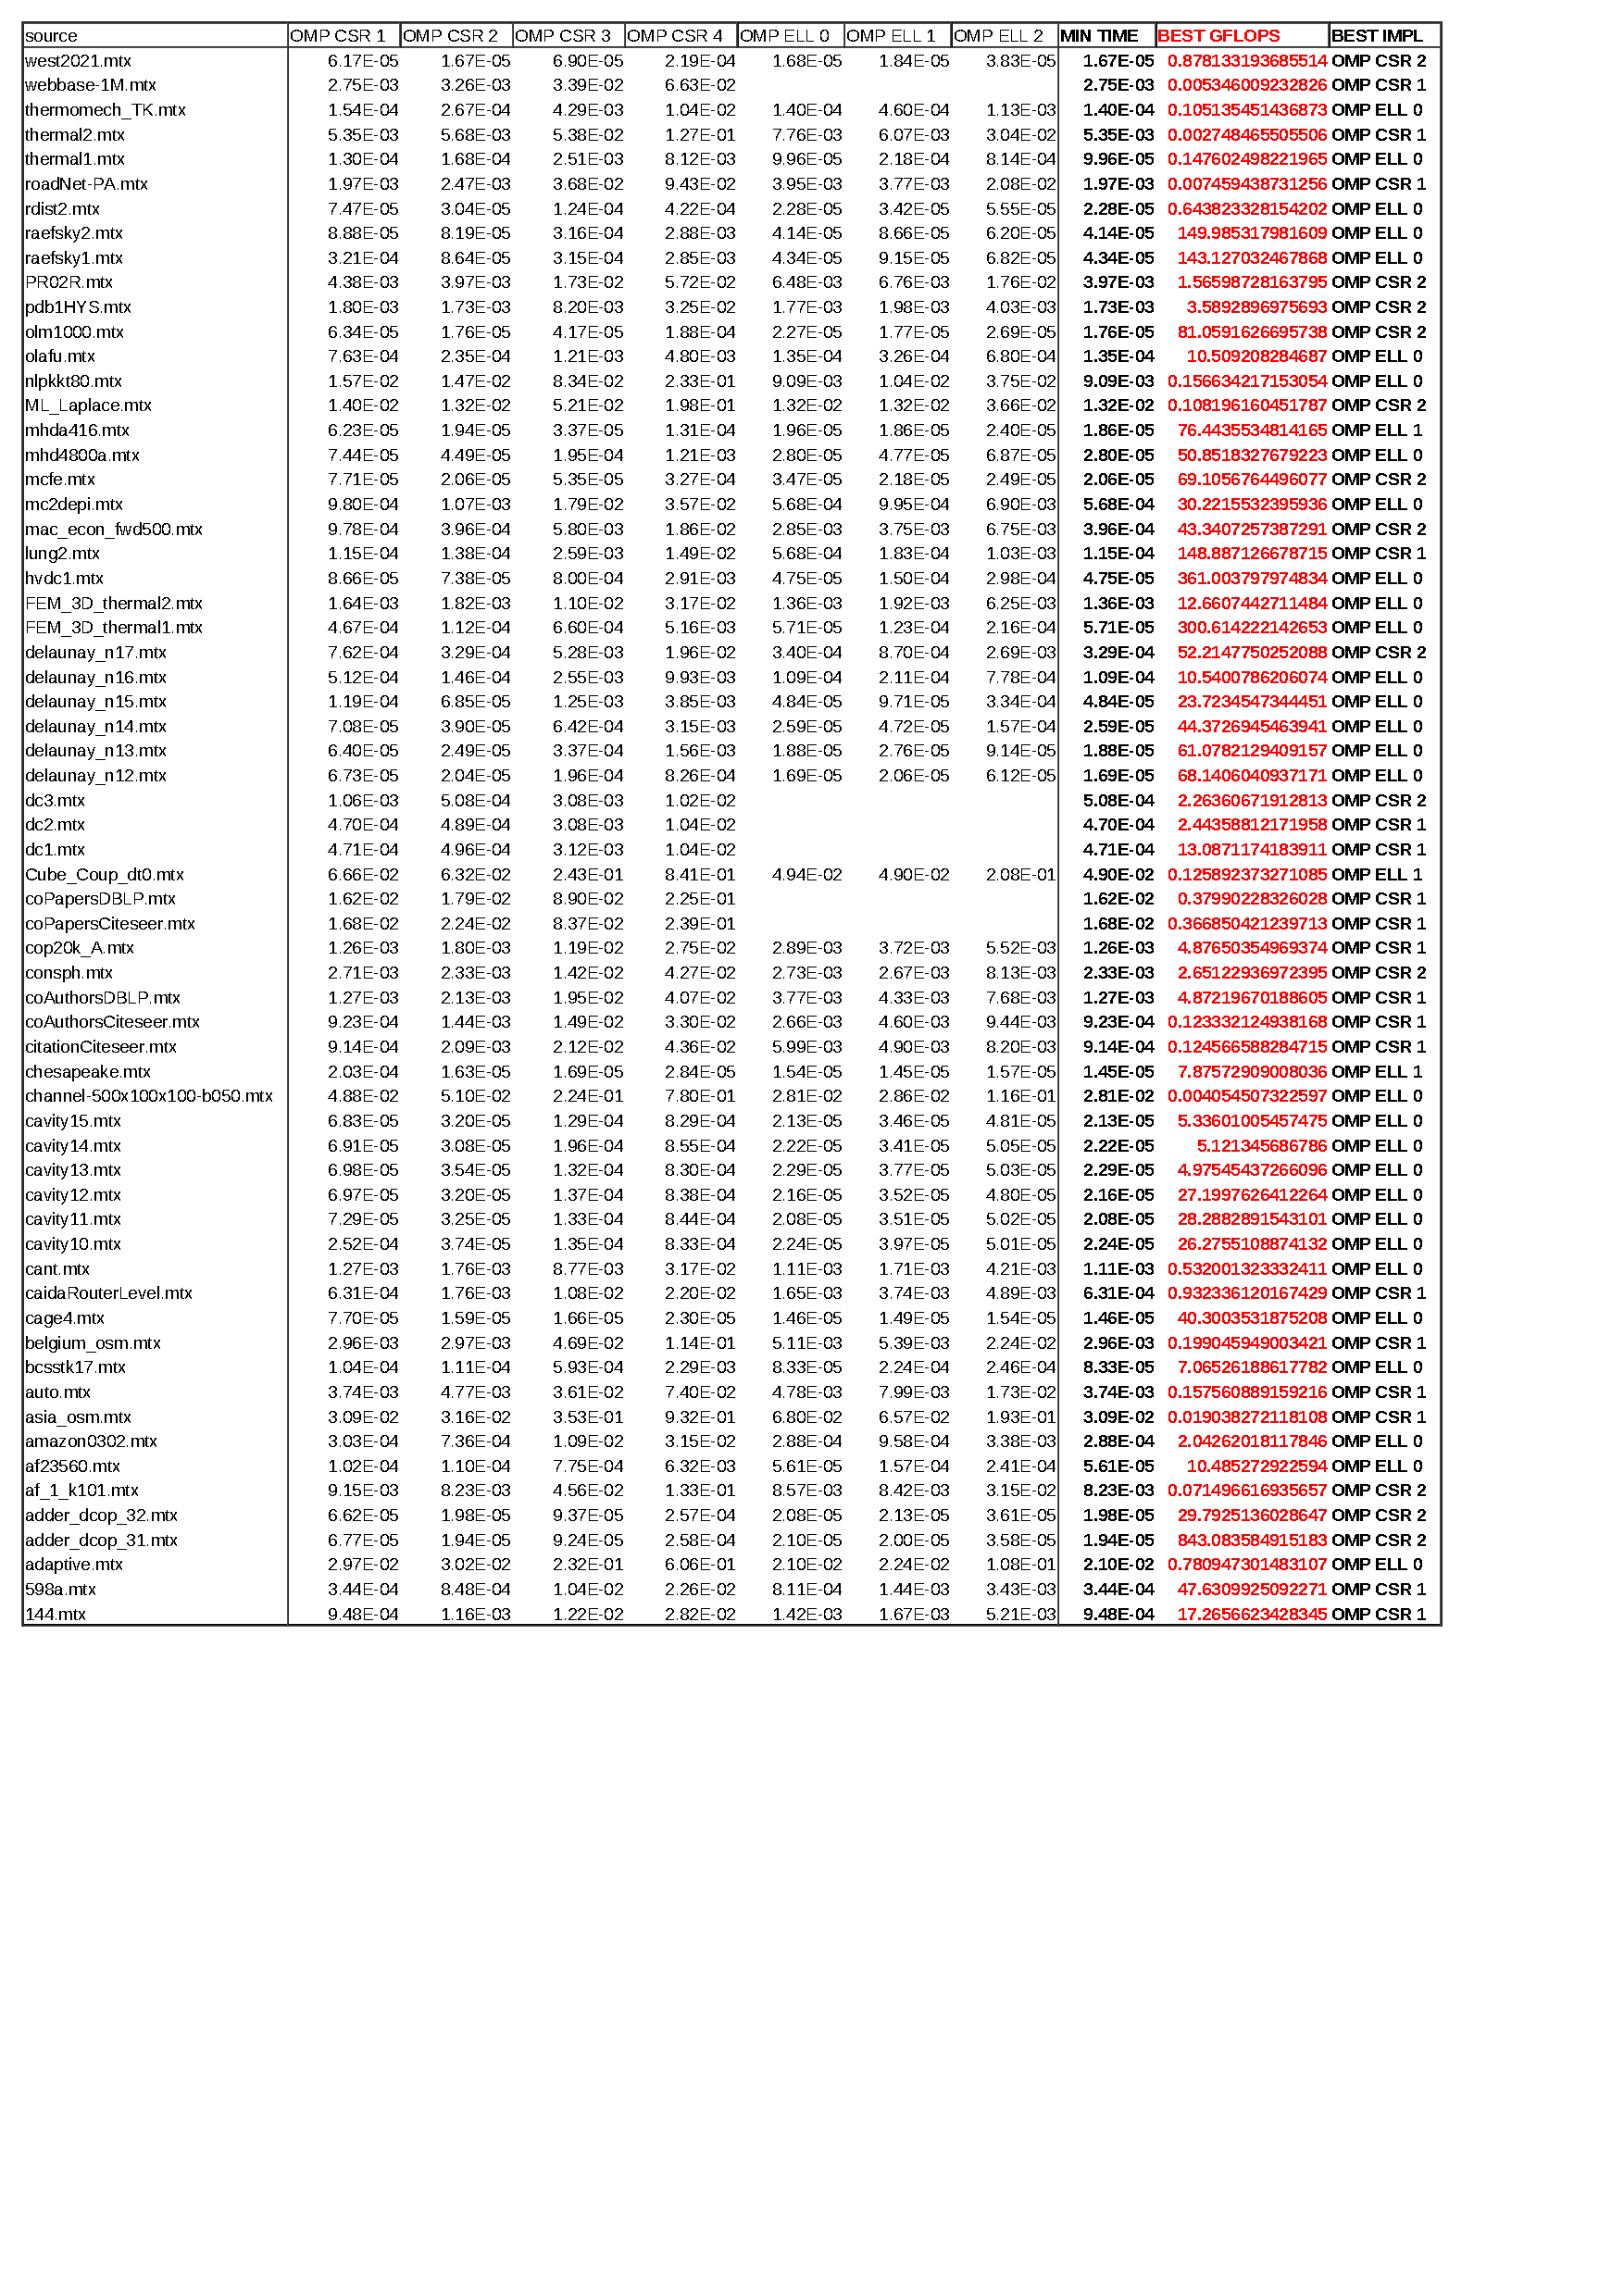
\includegraphics[width=\textwidth,height=\textheight,keepaspectratio=true]{ompNew_10x4_RL_NOSIMD_ImplConfrontoOut.pdf}
	%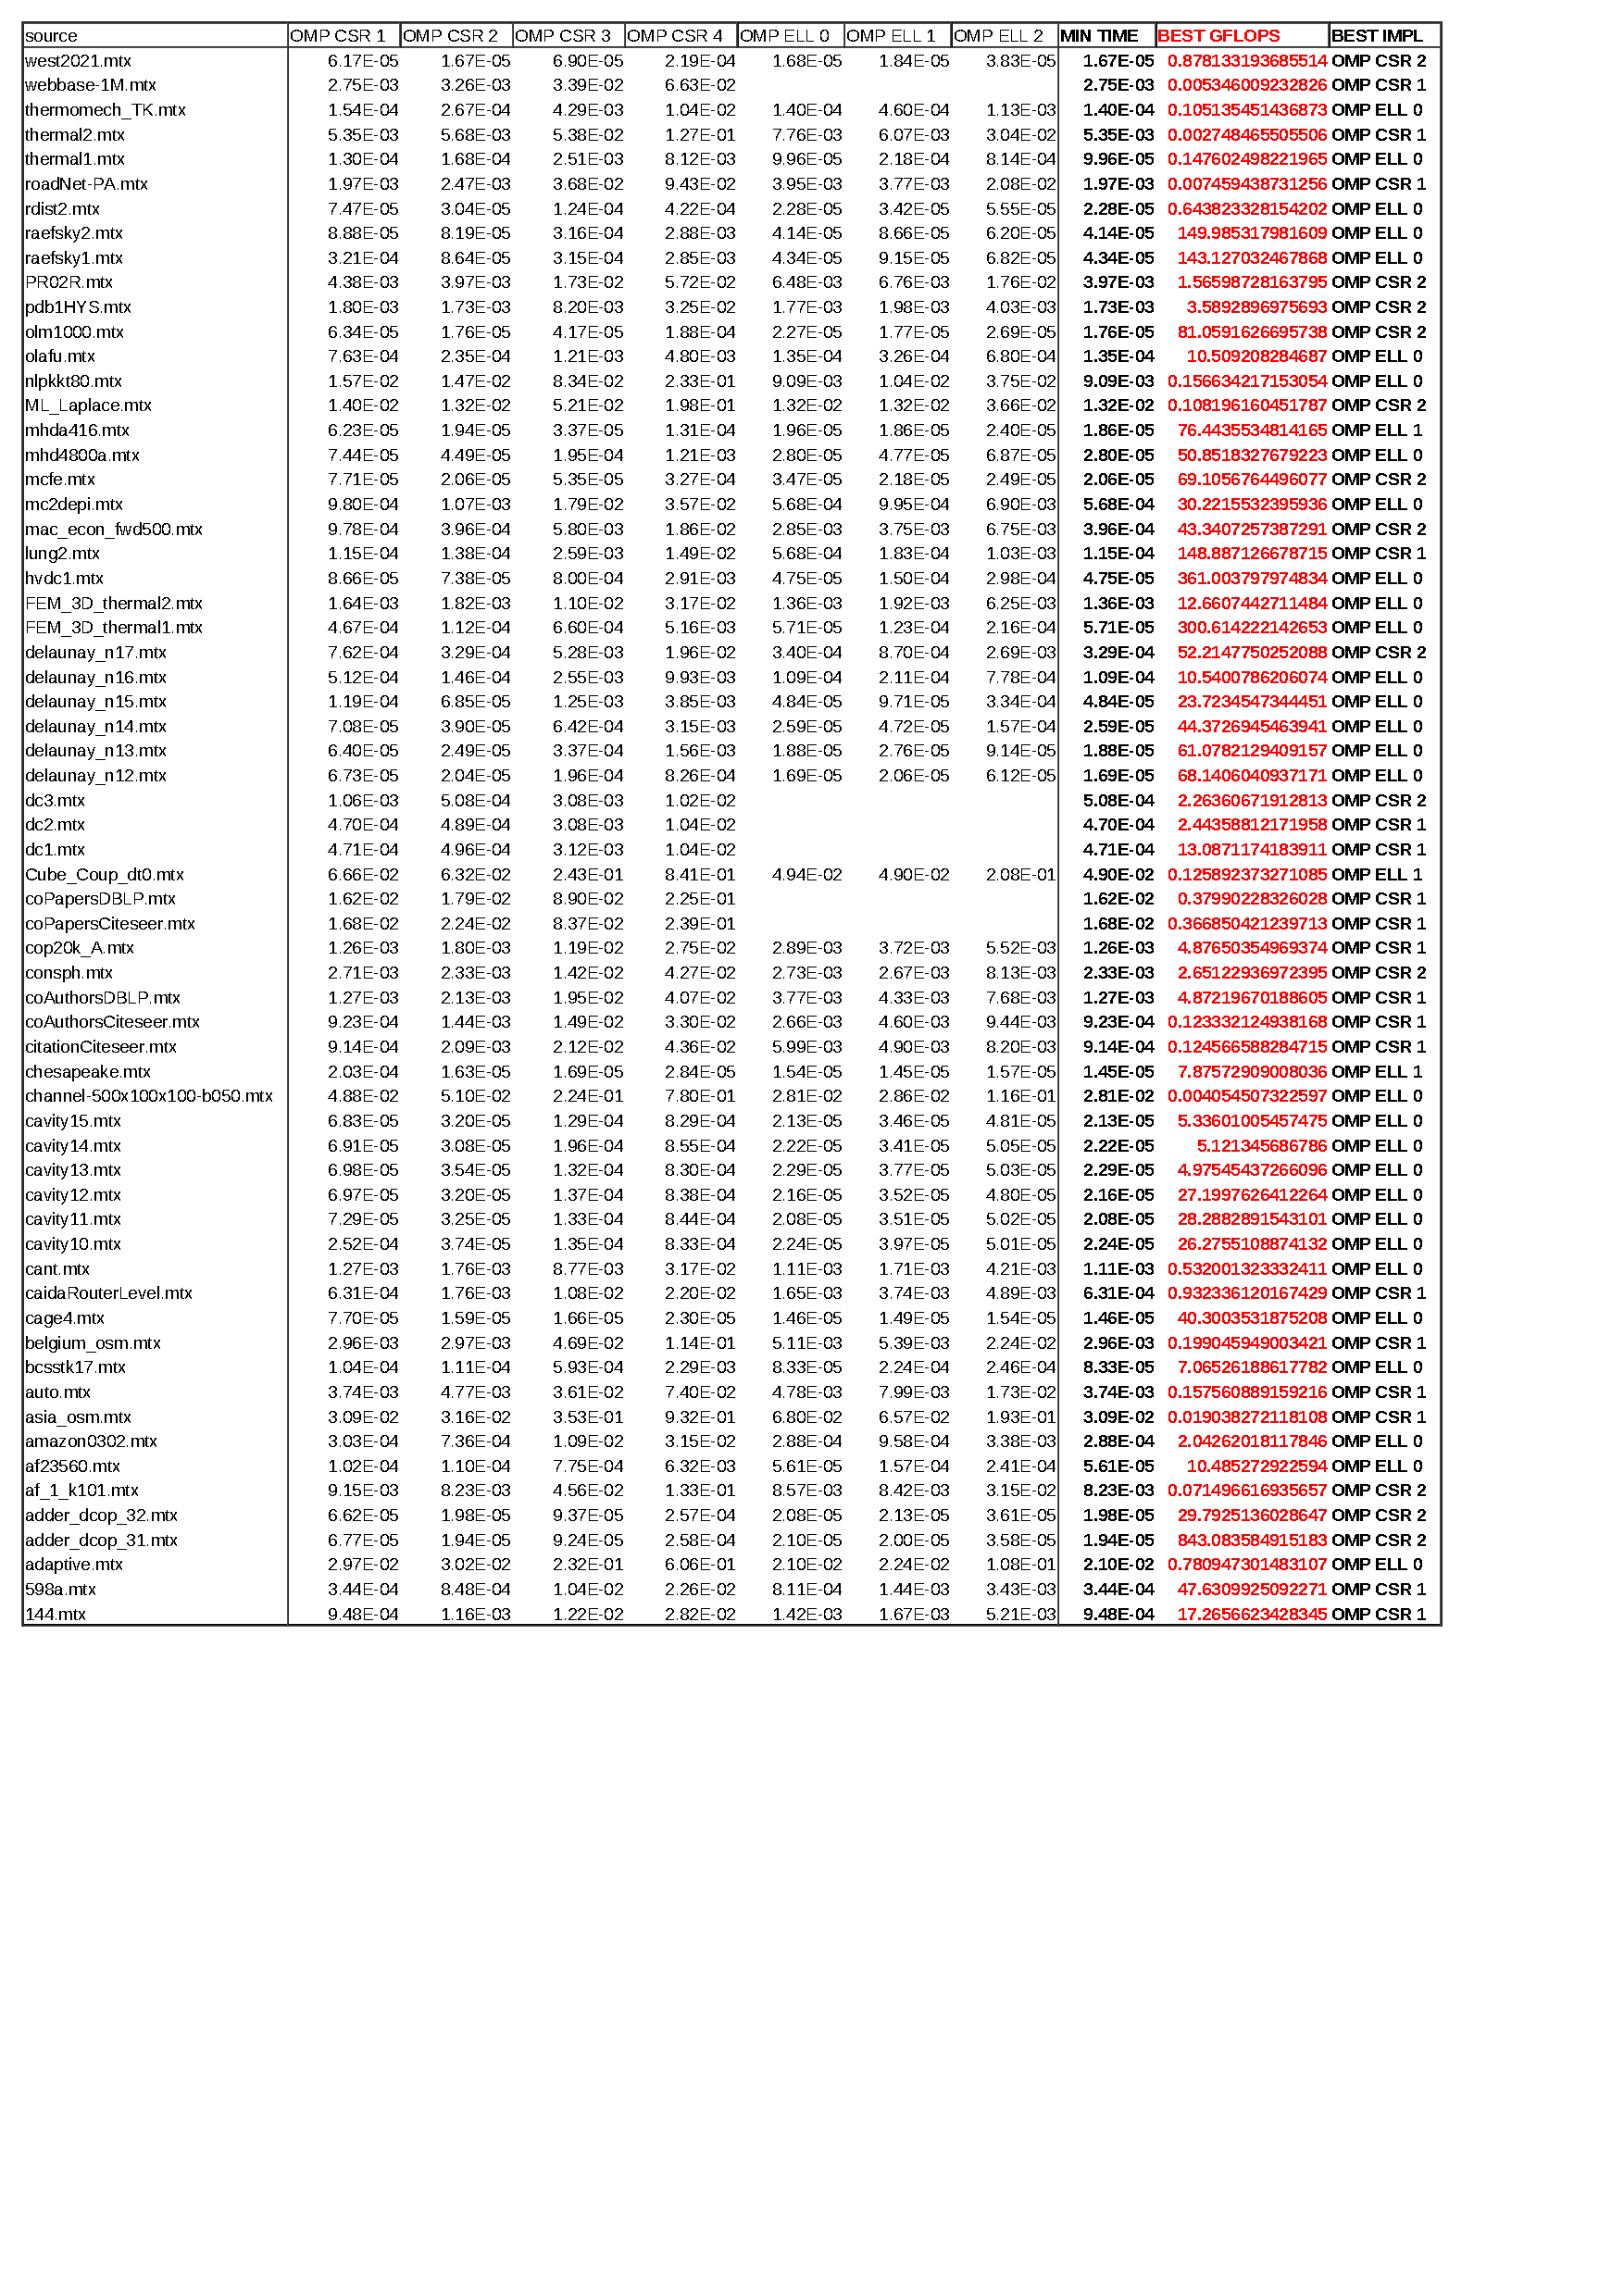
\includegraphics[scale=0.27]{ompNew_10x4_RL_NOSIMD_ImplConfrontoOut.pdf}
	\begin{figure}[h!]  \centering
        %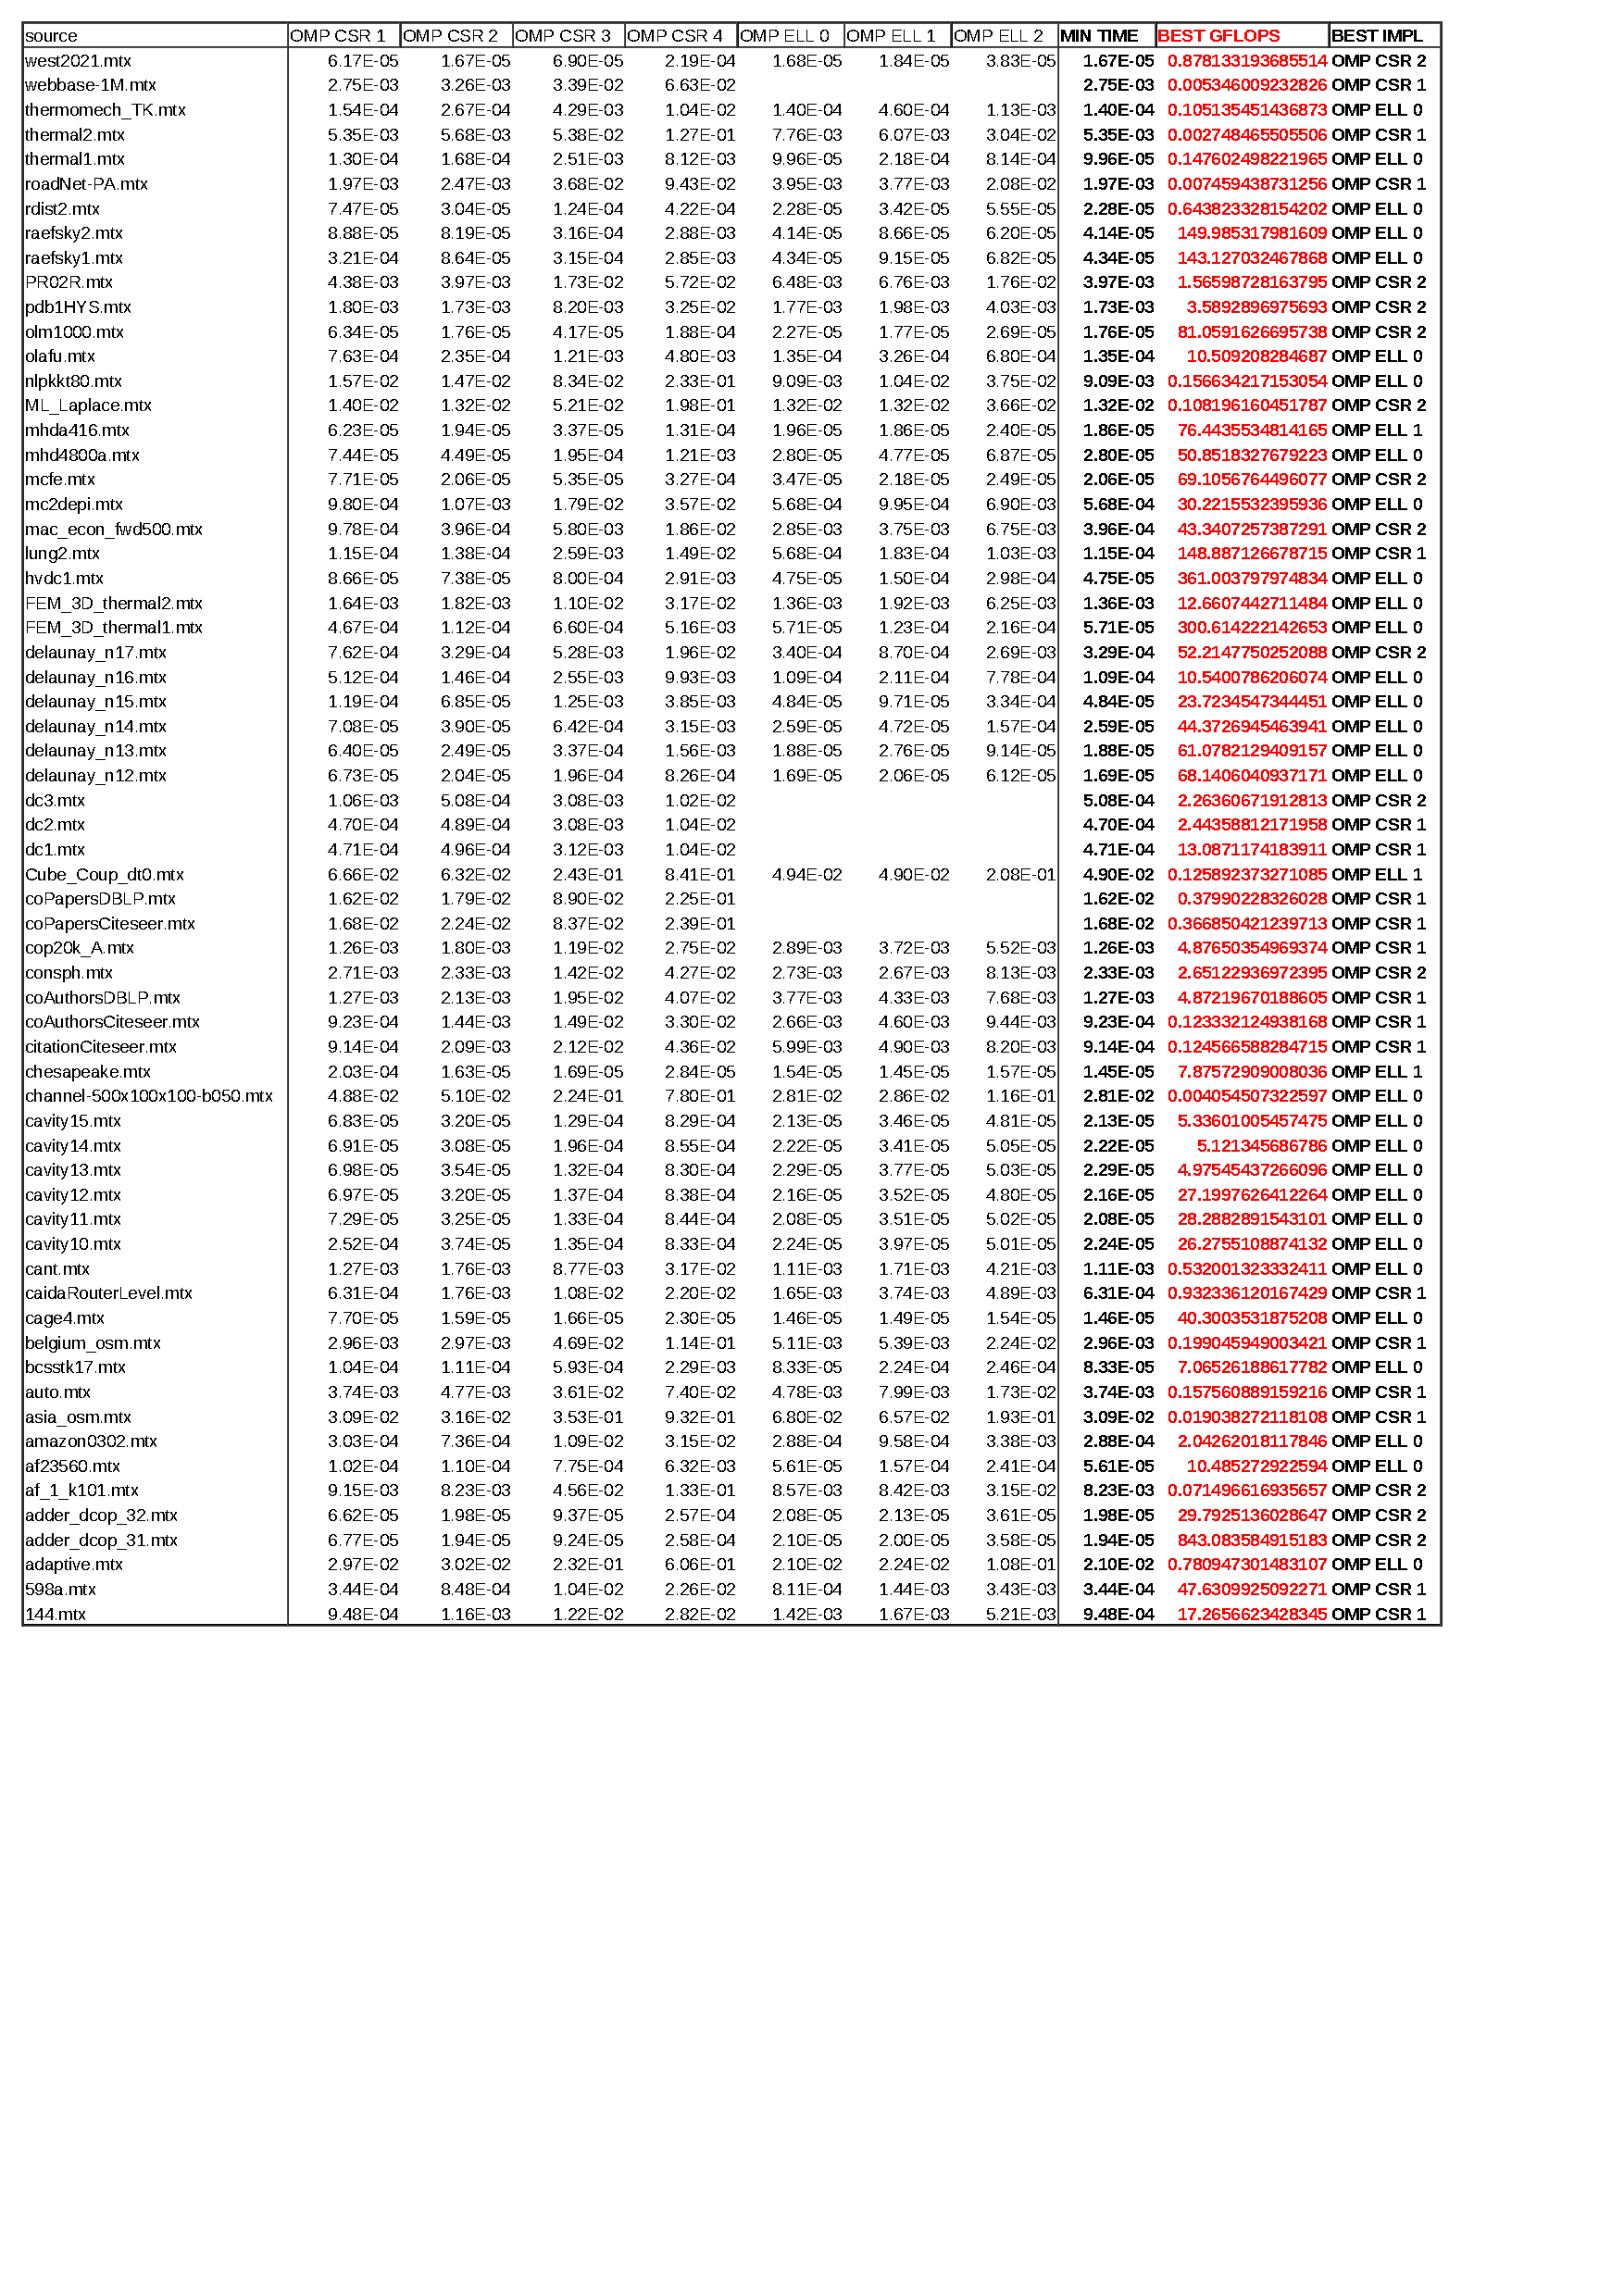
\includegraphics[width=\textwidth,height=\textheight,keepaspectratio=true]{ompNew_10x4_RL_NOSIMD_ImplConfrontoOut.pdf}
        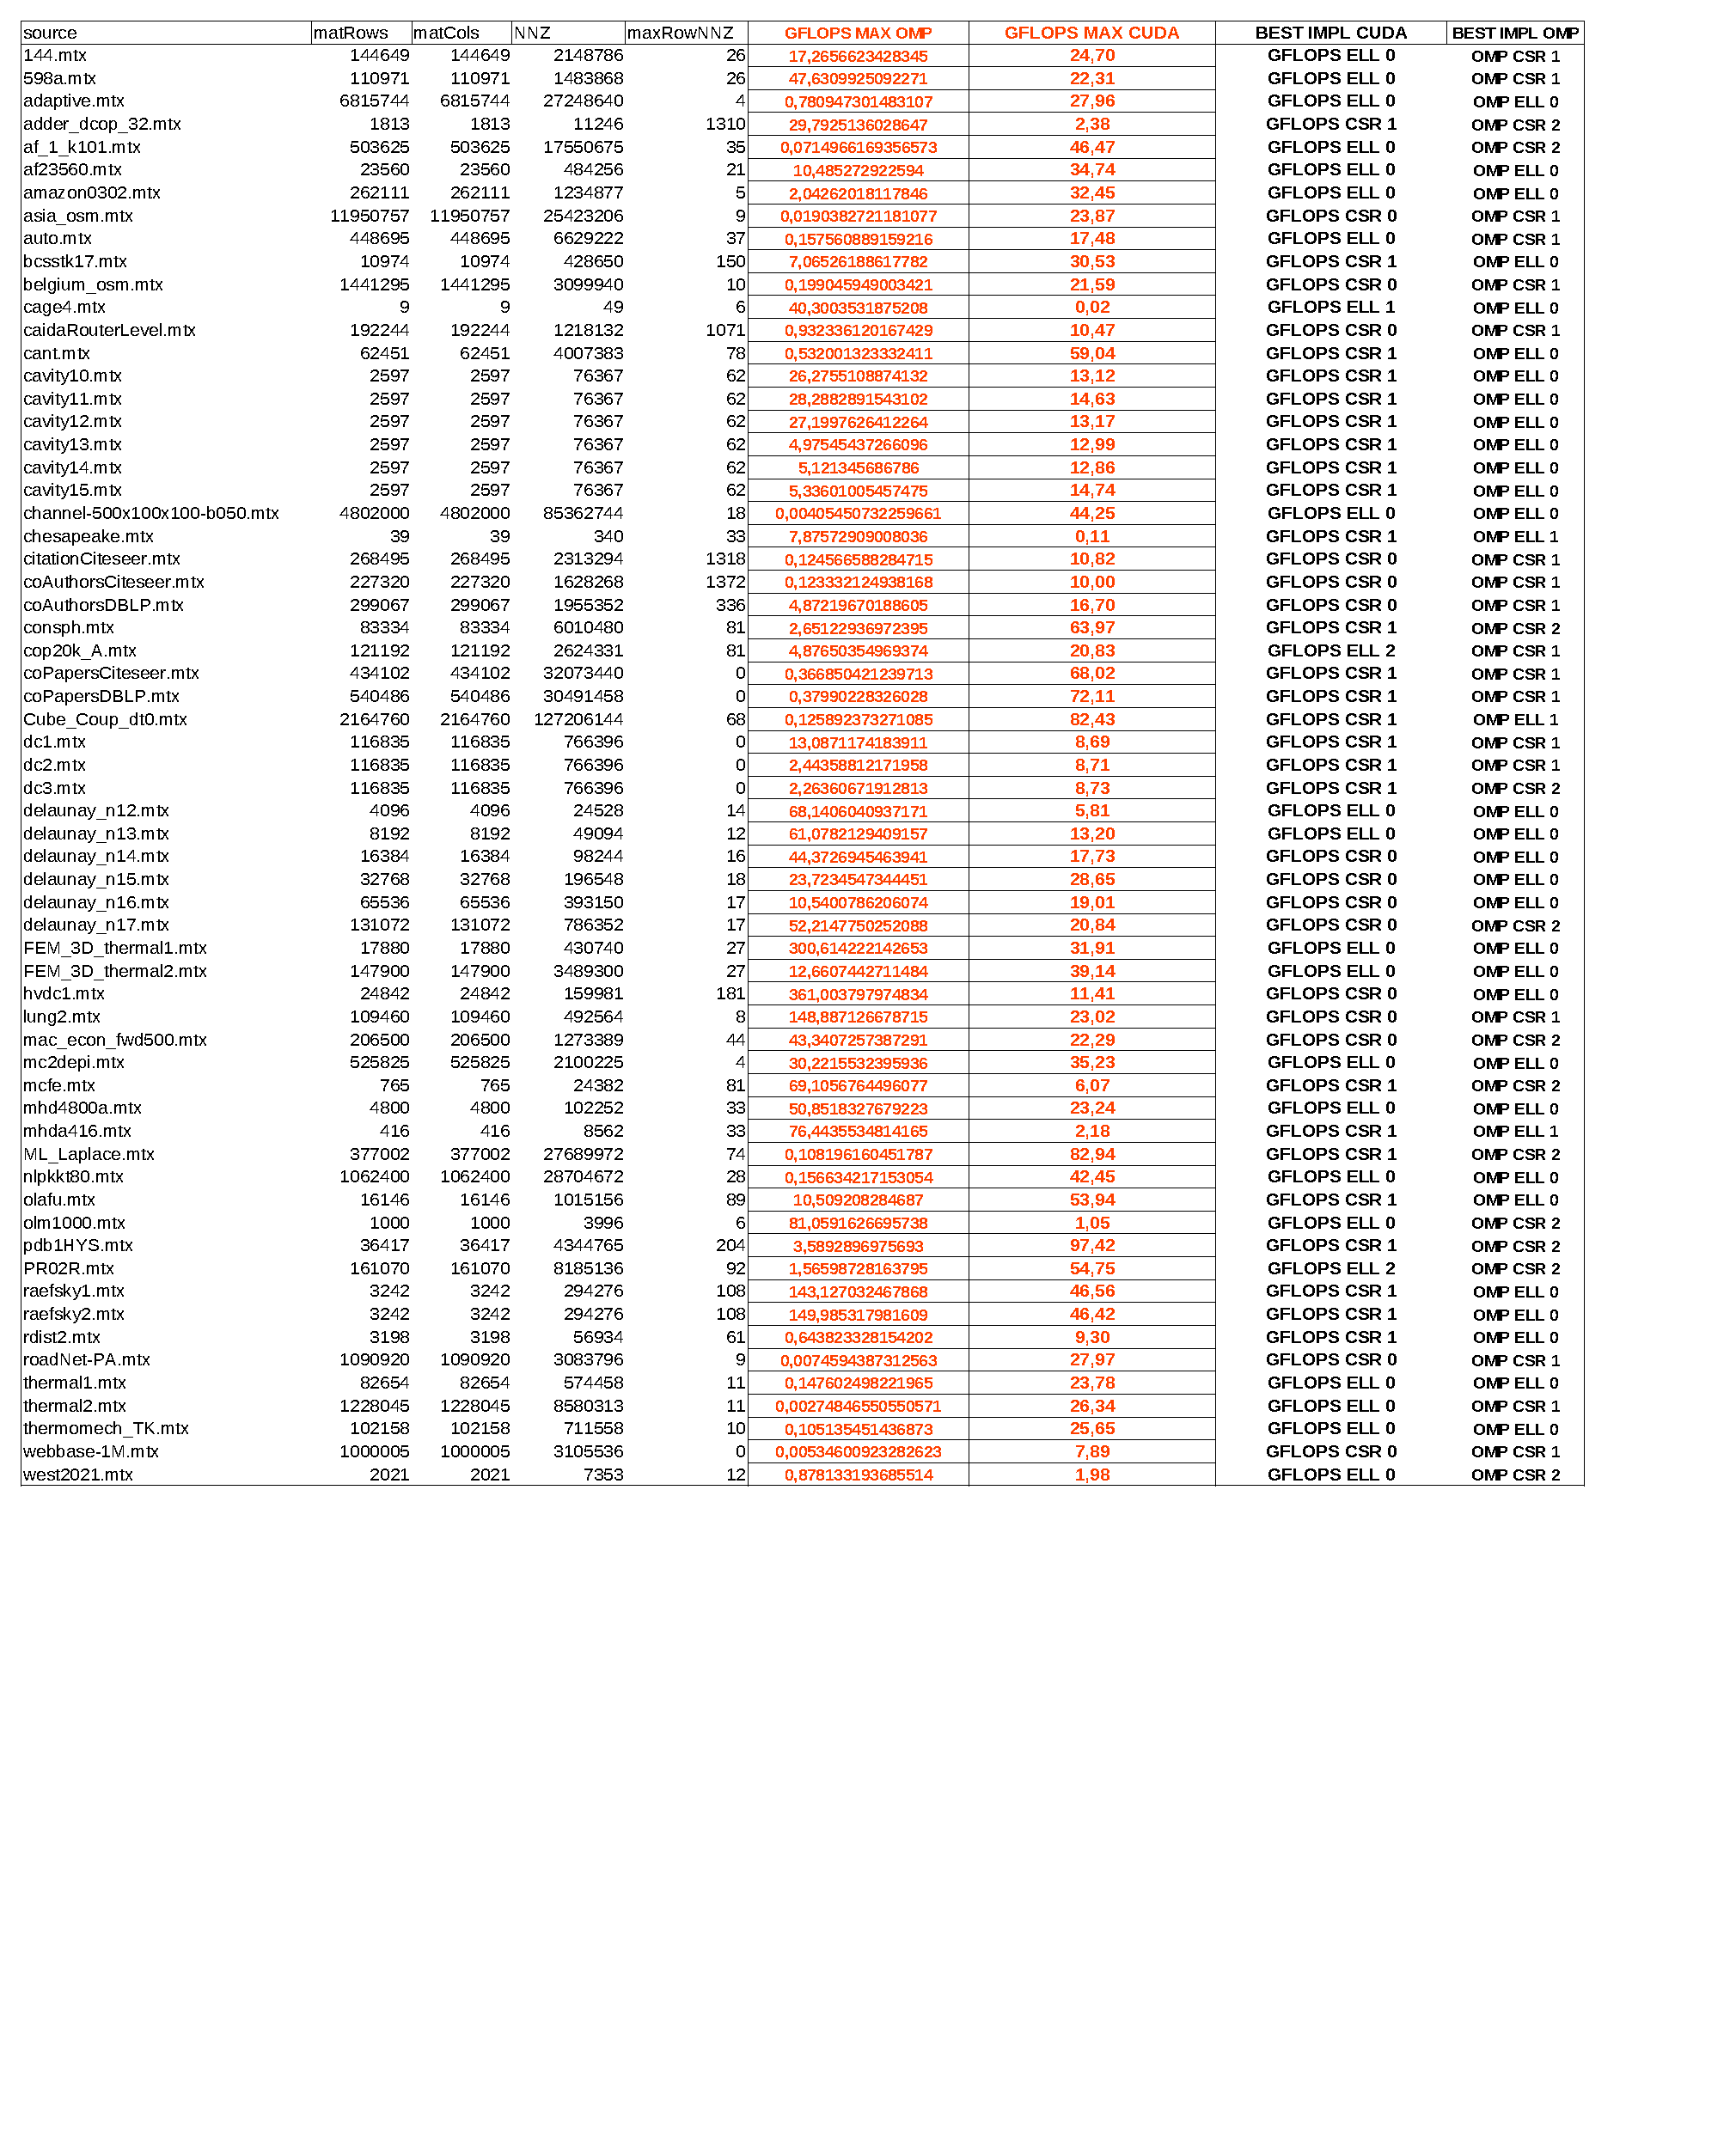
\includegraphics[scale=0.27]{cuda-ompConfronto.pdf}
        %\caption{pdf centering + width+height}
    \end{figure}
\end{frame}

\end{document}
